\renewcommand{\leveltopI}{-15cm + \leveltop}
\renewcommand{\leveltopII}{-15cm + \leveltopI}
\renewcommand{\leveltopIII}{-15cm + \leveltopII}
\renewcommand{\leveltopIIII}{-15cm + \leveltopIII}
\renewcommand{\leveltopIIIII}{-15cm + \leveltopIIII}
\renewcommand{\leveltopIIIIII}{-15cm + \leveltopIIIII}
\renewcommand{\leveltopIIIIIII}{-15cm + \leveltopIIIIII}
\renewcommand{\leveltopIIIIIIII}{-15cm + \leveltopIIIIIII}
\renewcommand{\leveltopIIIIIIIII}{-15cm + \leveltopIIIIIIII}
\renewcommand{\leveltopIIIIIIIIII}{-15cm + \leveltopIIIIIIIII}
\begin{tikzpicture}[scale=.2, anchor=south]
\begin{scope}[yshift=\leveltopI cm]
\matrix (line1) [column sep=1cm] {
\node[draw=black, rectangle split,  rectangle split parts=3] (sn0x21e1250){
\footnotesize{1}
\nodepart{two}
\begin{tikzpicture}[scale=.2]
\node[circle, scale=0.75, fill] (tid0) at (4.5,1.5){};
\node[circle, scale=0.75, fill] (tid1) at (2.25,3){};
\node[circle, scale=0.75, fill, red] (tid4) at (0.75,4.5){};
\node[circle, scale=0.75, fill, red] (tid5) at (2.25,4.5){};
\node[circle, scale=0.75, fill] (tid6) at (3.75,4.5){};
\draw[](tid1) -- (tid4);
\draw[](tid1) -- (tid5);
\draw[](tid1) -- (tid6);
\node[circle, scale=0.75, fill] (tid2) at (6,3){};
\node[circle, scale=0.75, fill] (tid7) at (5.25,4.5){};
\node[circle, scale=0.75, fill] (tid8) at (6.75,4.5){};
\draw[](tid2) -- (tid7);
\draw[](tid2) -- (tid8);
\node[circle, scale=0.75, fill] (tid3) at (8.25,3){};
\node[circle, scale=0.75, fill] (tid9) at (8.25,4.5){};
\draw[](tid3) -- (tid9);
\draw[](tid0) -- (tid1);
\draw[](tid0) -- (tid2);
\draw[](tid0) -- (tid3);
\end{tikzpicture}
\nodepart{three}
\footnotesize{6.125}
\nodepart{four}
\footnotesize{$25\:50\:25$}
};
 & 
\\
};
\end{scope}
\begin{scope}[yshift=\leveltopII cm]
\matrix (line2) [column sep=1cm] {
\node[draw=black, rectangle split,  rectangle split parts=3] (sn0x21e3370){
\footnotesize{0.25}
\nodepart{two}
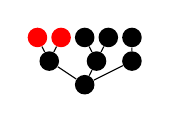
\begin{tikzpicture}[scale=.2]
\node[circle, scale=0.75, fill] (tid0) at (3.75,1.5){};
\node[circle, scale=0.75, fill] (tid1) at (1.5,3){};
\node[circle, scale=0.75, fill, red] (tid4) at (0.75,4.5){};
\node[circle, scale=0.75, fill, red] (tid5) at (2.25,4.5){};
\draw[](tid1) -- (tid4);
\draw[](tid1) -- (tid5);
\node[circle, scale=0.75, fill] (tid2) at (4.5,3){};
\node[circle, scale=0.75, fill] (tid6) at (3.75,4.5){};
\node[circle, scale=0.75, fill] (tid7) at (5.25,4.5){};
\draw[](tid2) -- (tid6);
\draw[](tid2) -- (tid7);
\node[circle, scale=0.75, fill] (tid3) at (6.75,3){};
\node[circle, scale=0.75, fill] (tid8) at (6.75,4.5){};
\draw[](tid3) -- (tid8);
\draw[](tid0) -- (tid1);
\draw[](tid0) -- (tid2);
\draw[](tid0) -- (tid3);
\end{tikzpicture}
\nodepart{three}
\footnotesize{5.625}
\nodepart{four}
\footnotesize{$67\:33$}
};
 & 
\node[draw=black, rectangle split,  rectangle split parts=3] (sn0x21e2ee0){
\footnotesize{0.5}
\nodepart{two}
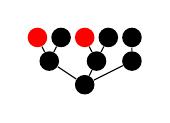
\begin{tikzpicture}[scale=.2]
\node[circle, scale=0.75, fill] (tid0) at (3.75,1.5){};
\node[circle, scale=0.75, fill] (tid1) at (1.5,3){};
\node[circle, scale=0.75, fill, red] (tid4) at (0.75,4.5){};
\node[circle, scale=0.75, fill] (tid5) at (2.25,4.5){};
\draw[](tid1) -- (tid4);
\draw[](tid1) -- (tid5);
\node[circle, scale=0.75, fill] (tid2) at (4.5,3){};
\node[circle, scale=0.75, fill, red] (tid6) at (3.75,4.5){};
\node[circle, scale=0.75, fill] (tid7) at (5.25,4.5){};
\draw[](tid2) -- (tid6);
\draw[](tid2) -- (tid7);
\node[circle, scale=0.75, fill] (tid3) at (6.75,3){};
\node[circle, scale=0.75, fill] (tid8) at (6.75,4.5){};
\draw[](tid3) -- (tid8);
\draw[](tid0) -- (tid1);
\draw[](tid0) -- (tid2);
\draw[](tid0) -- (tid3);
\end{tikzpicture}
\nodepart{three}
\footnotesize{5.625}
\nodepart{four}
\footnotesize{$67\:33$}
};
 & 
\node[draw=black, rectangle split,  rectangle split parts=3] (sn0x21e31c0){
\footnotesize{0.25}
\nodepart{two}
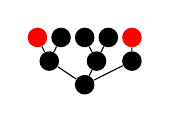
\begin{tikzpicture}[scale=.2]
\node[circle, scale=0.75, fill] (tid0) at (3.75,1.5){};
\node[circle, scale=0.75, fill] (tid1) at (1.5,3){};
\node[circle, scale=0.75, fill, red] (tid4) at (0.75,4.5){};
\node[circle, scale=0.75, fill] (tid5) at (2.25,4.5){};
\draw[](tid1) -- (tid4);
\draw[](tid1) -- (tid5);
\node[circle, scale=0.75, fill] (tid2) at (4.5,3){};
\node[circle, scale=0.75, fill] (tid6) at (3.75,4.5){};
\node[circle, scale=0.75, fill] (tid7) at (5.25,4.5){};
\draw[](tid2) -- (tid6);
\draw[](tid2) -- (tid7);
\node[circle, scale=0.75, fill] (tid3) at (6.75,3){};
\node[circle, scale=0.75, fill, red] (tid8) at (6.75,4.5){};
\draw[](tid3) -- (tid8);
\draw[](tid0) -- (tid1);
\draw[](tid0) -- (tid2);
\draw[](tid0) -- (tid3);
\end{tikzpicture}
\nodepart{three}
\footnotesize{5.625}
\nodepart{four}
\footnotesize{$33\:17\:17\:33$}
};
 & 
\\
};
\end{scope}
\begin{scope}[yshift=\leveltopIII cm]
\matrix (line3) [column sep=1cm] {
\node[draw=black, rectangle split,  rectangle split parts=3] (sn0x21e3fa0){
\footnotesize{0.583333}
\nodepart{two}
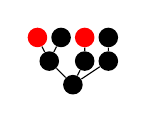
\begin{tikzpicture}[scale=.2]
\node[circle, scale=0.75, fill] (tid0) at (3,1.5){};
\node[circle, scale=0.75, fill] (tid1) at (1.5,3){};
\node[circle, scale=0.75, fill, red] (tid4) at (0.75,4.5){};
\node[circle, scale=0.75, fill] (tid5) at (2.25,4.5){};
\draw[](tid1) -- (tid4);
\draw[](tid1) -- (tid5);
\node[circle, scale=0.75, fill] (tid2) at (3.75,3){};
\node[circle, scale=0.75, fill, red] (tid6) at (3.75,4.5){};
\draw[](tid2) -- (tid6);
\node[circle, scale=0.75, fill] (tid3) at (5.25,3){};
\node[circle, scale=0.75, fill] (tid7) at (5.25,4.5){};
\draw[](tid3) -- (tid7);
\draw[](tid0) -- (tid1);
\draw[](tid0) -- (tid2);
\draw[](tid0) -- (tid3);
\end{tikzpicture}
\nodepart{three}
\footnotesize{5.125}
\nodepart{four}
\footnotesize{$50\:25\:25$}
};
 & 
\node[draw=black, rectangle split,  rectangle split parts=3] (sn0x21e4600){
\footnotesize{0.125}
\nodepart{two}
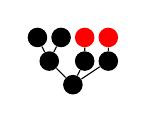
\begin{tikzpicture}[scale=.2]
\node[circle, scale=0.75, fill] (tid0) at (3,1.5){};
\node[circle, scale=0.75, fill] (tid1) at (1.5,3){};
\node[circle, scale=0.75, fill] (tid4) at (0.75,4.5){};
\node[circle, scale=0.75, fill] (tid5) at (2.25,4.5){};
\draw[](tid1) -- (tid4);
\draw[](tid1) -- (tid5);
\node[circle, scale=0.75, fill] (tid2) at (3.75,3){};
\node[circle, scale=0.75, fill, red] (tid6) at (3.75,4.5){};
\draw[](tid2) -- (tid6);
\node[circle, scale=0.75, fill] (tid3) at (5.25,3){};
\node[circle, scale=0.75, fill, red] (tid7) at (5.25,4.5){};
\draw[](tid3) -- (tid7);
\draw[](tid0) -- (tid1);
\draw[](tid0) -- (tid2);
\draw[](tid0) -- (tid3);
\end{tikzpicture}
\nodepart{three}
\footnotesize{5.125}
\nodepart{four}
\footnotesize{$1$}
};
 & 
\node[draw=black, rectangle split,  rectangle split parts=3] (sn0x21e7270){
\footnotesize{0.166667}
\nodepart{two}
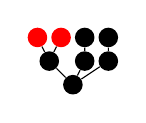
\begin{tikzpicture}[scale=.2]
\node[circle, scale=0.75, fill] (tid0) at (3,1.5){};
\node[circle, scale=0.75, fill] (tid1) at (1.5,3){};
\node[circle, scale=0.75, fill, red] (tid4) at (0.75,4.5){};
\node[circle, scale=0.75, fill, red] (tid5) at (2.25,4.5){};
\draw[](tid1) -- (tid4);
\draw[](tid1) -- (tid5);
\node[circle, scale=0.75, fill] (tid2) at (3.75,3){};
\node[circle, scale=0.75, fill] (tid6) at (3.75,4.5){};
\draw[](tid2) -- (tid6);
\node[circle, scale=0.75, fill] (tid3) at (5.25,3){};
\node[circle, scale=0.75, fill] (tid7) at (5.25,4.5){};
\draw[](tid3) -- (tid7);
\draw[](tid0) -- (tid1);
\draw[](tid0) -- (tid2);
\draw[](tid0) -- (tid3);
\end{tikzpicture}
\nodepart{three}
\footnotesize{5.125}
\nodepart{four}
\footnotesize{$1$}
};
 & 
\node[draw=black, rectangle split,  rectangle split parts=3] (sn0x21e79c0){
\footnotesize{0.0416667}
\nodepart{two}
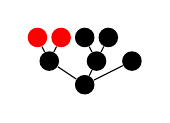
\begin{tikzpicture}[scale=.2]
\node[circle, scale=0.75, fill] (tid0) at (3.75,1.5){};
\node[circle, scale=0.75, fill] (tid1) at (1.5,3){};
\node[circle, scale=0.75, fill, red] (tid4) at (0.75,4.5){};
\node[circle, scale=0.75, fill, red] (tid5) at (2.25,4.5){};
\draw[](tid1) -- (tid4);
\draw[](tid1) -- (tid5);
\node[circle, scale=0.75, fill] (tid2) at (4.5,3){};
\node[circle, scale=0.75, fill] (tid6) at (3.75,4.5){};
\node[circle, scale=0.75, fill] (tid7) at (5.25,4.5){};
\draw[](tid2) -- (tid6);
\draw[](tid2) -- (tid7);
\node[circle, scale=0.75, fill] (tid3) at (6.75,3){};
\draw[](tid0) -- (tid1);
\draw[](tid0) -- (tid2);
\draw[](tid0) -- (tid3);
\end{tikzpicture}
\nodepart{three}
\footnotesize{5.125}
\nodepart{four}
\footnotesize{$1$}
};
 & 
\node[draw=black, rectangle split,  rectangle split parts=3] (sn0x21e6f50){
\footnotesize{0.0833333}
\nodepart{two}
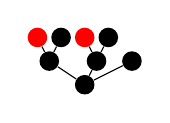
\begin{tikzpicture}[scale=.2]
\node[circle, scale=0.75, fill] (tid0) at (3.75,1.5){};
\node[circle, scale=0.75, fill] (tid1) at (1.5,3){};
\node[circle, scale=0.75, fill, red] (tid4) at (0.75,4.5){};
\node[circle, scale=0.75, fill] (tid5) at (2.25,4.5){};
\draw[](tid1) -- (tid4);
\draw[](tid1) -- (tid5);
\node[circle, scale=0.75, fill] (tid2) at (4.5,3){};
\node[circle, scale=0.75, fill, red] (tid6) at (3.75,4.5){};
\node[circle, scale=0.75, fill] (tid7) at (5.25,4.5){};
\draw[](tid2) -- (tid6);
\draw[](tid2) -- (tid7);
\node[circle, scale=0.75, fill] (tid3) at (6.75,3){};
\draw[](tid0) -- (tid1);
\draw[](tid0) -- (tid2);
\draw[](tid0) -- (tid3);
\end{tikzpicture}
\nodepart{three}
\footnotesize{5.125}
\nodepart{four}
\footnotesize{$50\:50$}
};
 & 
\\
};
\end{scope}
\begin{scope}[yshift=\leveltopIIII cm]
\matrix (line4) [column sep=1cm] {
\node[draw=black, rectangle split,  rectangle split parts=3] (sn0x21e4440){
\footnotesize{0.458333}
\nodepart{two}
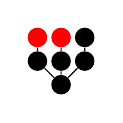
\begin{tikzpicture}[scale=.2]
\node[circle, scale=0.75, fill] (tid0) at (2.25,1.5){};
\node[circle, scale=0.75, fill] (tid1) at (0.75,3){};
\node[circle, scale=0.75, fill, red] (tid4) at (0.75,4.5){};
\draw[](tid1) -- (tid4);
\node[circle, scale=0.75, fill] (tid2) at (2.25,3){};
\node[circle, scale=0.75, fill, red] (tid5) at (2.25,4.5){};
\draw[](tid2) -- (tid5);
\node[circle, scale=0.75, fill] (tid3) at (3.75,3){};
\node[circle, scale=0.75, fill] (tid6) at (3.75,4.5){};
\draw[](tid3) -- (tid6);
\draw[](tid0) -- (tid1);
\draw[](tid0) -- (tid2);
\draw[](tid0) -- (tid3);
\end{tikzpicture}
\nodepart{three}
\footnotesize{4.625}
\nodepart{four}
\footnotesize{$1$}
};
 & 
\node[draw=black, rectangle split,  rectangle split parts=3] (sn0x21e48e0){
\footnotesize{0.1875}
\nodepart{two}
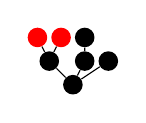
\begin{tikzpicture}[scale=.2]
\node[circle, scale=0.75, fill] (tid0) at (3,1.5){};
\node[circle, scale=0.75, fill] (tid1) at (1.5,3){};
\node[circle, scale=0.75, fill, red] (tid4) at (0.75,4.5){};
\node[circle, scale=0.75, fill, red] (tid5) at (2.25,4.5){};
\draw[](tid1) -- (tid4);
\draw[](tid1) -- (tid5);
\node[circle, scale=0.75, fill] (tid2) at (3.75,3){};
\node[circle, scale=0.75, fill] (tid6) at (3.75,4.5){};
\draw[](tid2) -- (tid6);
\node[circle, scale=0.75, fill] (tid3) at (5.25,3){};
\draw[](tid0) -- (tid1);
\draw[](tid0) -- (tid2);
\draw[](tid0) -- (tid3);
\end{tikzpicture}
\nodepart{three}
\footnotesize{4.625}
\nodepart{four}
\footnotesize{$1$}
};
 & 
\node[draw=black, rectangle split,  rectangle split parts=3] (sn0x21e49b0){
\footnotesize{0.354167}
\nodepart{two}
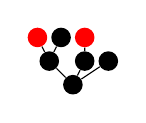
\begin{tikzpicture}[scale=.2]
\node[circle, scale=0.75, fill] (tid0) at (3,1.5){};
\node[circle, scale=0.75, fill] (tid1) at (1.5,3){};
\node[circle, scale=0.75, fill, red] (tid4) at (0.75,4.5){};
\node[circle, scale=0.75, fill] (tid5) at (2.25,4.5){};
\draw[](tid1) -- (tid4);
\draw[](tid1) -- (tid5);
\node[circle, scale=0.75, fill] (tid2) at (3.75,3){};
\node[circle, scale=0.75, fill, red] (tid6) at (3.75,4.5){};
\draw[](tid2) -- (tid6);
\node[circle, scale=0.75, fill] (tid3) at (5.25,3){};
\draw[](tid0) -- (tid1);
\draw[](tid0) -- (tid2);
\draw[](tid0) -- (tid3);
\end{tikzpicture}
\nodepart{three}
\footnotesize{4.625}
\nodepart{four}
\footnotesize{$50\:50$}
};
 & 
\\
};
\end{scope}
\begin{scope}[yshift=\leveltopIIIII cm]
\matrix (line5) [column sep=1cm] {
\node[draw=black, rectangle split,  rectangle split parts=3] (sn0x21e5140){
\footnotesize{0.822917}
\nodepart{two}
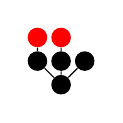
\begin{tikzpicture}[scale=.2]
\node[circle, scale=0.75, fill] (tid0) at (2.25,1.5){};
\node[circle, scale=0.75, fill] (tid1) at (0.75,3){};
\node[circle, scale=0.75, fill, red] (tid4) at (0.75,4.5){};
\draw[](tid1) -- (tid4);
\node[circle, scale=0.75, fill] (tid2) at (2.25,3){};
\node[circle, scale=0.75, fill, red] (tid5) at (2.25,4.5){};
\draw[](tid2) -- (tid5);
\node[circle, scale=0.75, fill] (tid3) at (3.75,3){};
\draw[](tid0) -- (tid1);
\draw[](tid0) -- (tid2);
\draw[](tid0) -- (tid3);
\end{tikzpicture}
\nodepart{three}
\footnotesize{4.125}
\nodepart{four}
\footnotesize{$1$}
};
 & 
\node[draw=black, rectangle split,  rectangle split parts=3] (sn0x21e5e90){
\footnotesize{0.177083}
\nodepart{two}
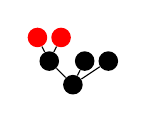
\begin{tikzpicture}[scale=.2]
\node[circle, scale=0.75, fill] (tid0) at (3,1.5){};
\node[circle, scale=0.75, fill] (tid1) at (1.5,3){};
\node[circle, scale=0.75, fill, red] (tid4) at (0.75,4.5){};
\node[circle, scale=0.75, fill, red] (tid5) at (2.25,4.5){};
\draw[](tid1) -- (tid4);
\draw[](tid1) -- (tid5);
\node[circle, scale=0.75, fill] (tid2) at (3.75,3){};
\node[circle, scale=0.75, fill] (tid3) at (5.25,3){};
\draw[](tid0) -- (tid1);
\draw[](tid0) -- (tid2);
\draw[](tid0) -- (tid3);
\end{tikzpicture}
\nodepart{three}
\footnotesize{4.125}
\nodepart{four}
\footnotesize{$1$}
};
 & 
\\
};
\end{scope}
\begin{scope}[yshift=\leveltopIIIIII cm]
\matrix (line6) [column sep=1cm] {
\node[draw=black, rectangle split,  rectangle split parts=3] (sn0x21e5300){
\footnotesize{1}
\nodepart{two}
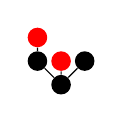
\begin{tikzpicture}[scale=.2]
\node[circle, scale=0.75, fill] (tid0) at (2.25,1.5){};
\node[circle, scale=0.75, fill] (tid1) at (0.75,3){};
\node[circle, scale=0.75, fill, red] (tid4) at (0.75,4.5){};
\draw[](tid1) -- (tid4);
\node[circle, scale=0.75, fill, red] (tid2) at (2.25,3){};
\node[circle, scale=0.75, fill] (tid3) at (3.75,3){};
\draw[](tid0) -- (tid1);
\draw[](tid0) -- (tid2);
\draw[](tid0) -- (tid3);
\end{tikzpicture}
\nodepart{three}
\footnotesize{3.625}
\nodepart{four}
\footnotesize{$50\:50$}
};
 & 
\\
};
\end{scope}
\begin{scope}[yshift=\leveltopIIIIIII cm]
\matrix (line7) [column sep=1cm] {
\node[draw=black, rectangle split,  rectangle split parts=3] (sn0x21e4eb0){
\footnotesize{0.5}
\nodepart{two}
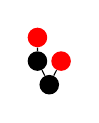
\begin{tikzpicture}[scale=.2]
\node[circle, scale=0.75, fill] (tid0) at (1.5,1.5){};
\node[circle, scale=0.75, fill] (tid1) at (0.75,3){};
\node[circle, scale=0.75, fill, red] (tid3) at (0.75,4.5){};
\draw[](tid1) -- (tid3);
\node[circle, scale=0.75, fill, red] (tid2) at (2.25,3){};
\draw[](tid0) -- (tid1);
\draw[](tid0) -- (tid2);
\end{tikzpicture}
\nodepart{three}
\footnotesize{3.25}
\nodepart{four}
\footnotesize{$50\:50$}
};
 & 
\node[draw=black, rectangle split,  rectangle split parts=3] (sn0x21e57b0){
\footnotesize{0.5}
\nodepart{two}
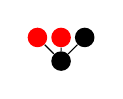
\begin{tikzpicture}[scale=.2]
\node[circle, scale=0.75, fill] (tid0) at (2.25,1.5){};
\node[circle, scale=0.75, fill, red] (tid1) at (0.75,3){};
\node[circle, scale=0.75, fill, red] (tid2) at (2.25,3){};
\node[circle, scale=0.75, fill] (tid3) at (3.75,3){};
\draw[](tid0) -- (tid1);
\draw[](tid0) -- (tid2);
\draw[](tid0) -- (tid3);
\end{tikzpicture}
\nodepart{three}
\footnotesize{3}
\nodepart{four}
\footnotesize{$1$}
};
 & 
\\
};
\end{scope}
\begin{scope}[yshift=\leveltopIIIIIIII cm]
\matrix (line8) [column sep=1cm] {
\node[draw=black, rectangle split,  rectangle split parts=3] (sn0x21e5880){
\footnotesize{0.25}
\nodepart{two}
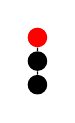
\begin{tikzpicture}[scale=.2]
\node[circle, scale=0.75, fill] (tid0) at (0.75,1.5){};
\node[circle, scale=0.75, fill] (tid1) at (0.75,3){};
\node[circle, scale=0.75, fill, red] (tid2) at (0.75,4.5){};
\draw[](tid1) -- (tid2);
\draw[](tid0) -- (tid1);
\end{tikzpicture}
\nodepart{three}
\footnotesize{3}
\nodepart{four}
\footnotesize{$1$}
};
 & 
\node[draw=black, rectangle split,  rectangle split parts=3] (sn0x21e5950){
\footnotesize{0.75}
\nodepart{two}

\begin{tikzpicture}[scale=.2]
\node[circle, scale=0.75, fill] (tid0) at (1.5,1.5){};
\node[circle, scale=0.75, fill, red] (tid1) at (0.75,3){};
\node[circle, scale=0.75, fill, red] (tid2) at (2.25,3){};
\draw[](tid0) -- (tid1);
\draw[](tid0) -- (tid2);
\end{tikzpicture}
\nodepart{three}
\footnotesize{2.5}
\nodepart{four}
\footnotesize{$1$}
};
 & 
\\
};
\end{scope}
\begin{scope}[yshift=\leveltopIIIIIIIII cm]
\matrix (line9) [column sep=1cm] {
\node[draw=black, rectangle split,  rectangle split parts=3] (sn0x21e5a20){
\footnotesize{1}
\nodepart{two}

\begin{tikzpicture}[scale=.2]
\node[circle, scale=0.75, fill] (tid0) at (0.75,1.5){};
\node[circle, scale=0.75, fill, red] (tid1) at (0.75,3){};
\draw[](tid0) -- (tid1);
\end{tikzpicture}
\nodepart{three}
\footnotesize{2}
\nodepart{four}
\footnotesize{$1$}
};
 & 
\\
};
\end{scope}
\begin{scope}[yshift=\leveltopIIIIIIIIII cm]
\matrix (line10) [column sep=1cm] {
\node[draw=black, rectangle split,  rectangle split parts=3] (sn0x21e5af0){
\footnotesize{1}
\nodepart{two}

\begin{tikzpicture}[scale=.2]
\node[circle, scale=0.75, fill, red] (tid0) at (0.75,1.5){};
\end{tikzpicture}
\nodepart{three}
\footnotesize{1}
\nodepart{four}
\footnotesize{$$}
};
 & 
\\
};
\end{scope}
\begin{scope}[yshift=\leveltopIIIIIIIIIII cm]
\matrix (line11) [column sep=1cm] {
\\
};
\end{scope}
\draw (sn0x21e1250.south) -- (sn0x21e3370.north);
\draw (sn0x21e1250.south) -- (sn0x21e2ee0.north);
\draw (sn0x21e1250.south) -- (sn0x21e31c0.north);
\draw (sn0x21e3370.south) -- (sn0x21e3fa0.north);
\draw (sn0x21e3370.south) -- (sn0x21e4600.north);
\draw (sn0x21e2ee0.south) -- (sn0x21e3fa0.north);
\draw (sn0x21e2ee0.south) -- (sn0x21e7270.north);
\draw (sn0x21e31c0.south) -- (sn0x21e4600.north);
\draw (sn0x21e31c0.south) -- (sn0x21e3fa0.north);
\draw (sn0x21e31c0.south) -- (sn0x21e79c0.north);
\draw (sn0x21e31c0.south) -- (sn0x21e6f50.north);
\draw (sn0x21e3fa0.south) -- (sn0x21e4440.north);
\draw (sn0x21e3fa0.south) -- (sn0x21e48e0.north);
\draw (sn0x21e3fa0.south) -- (sn0x21e49b0.north);
\draw (sn0x21e4600.south) -- (sn0x21e49b0.north);
\draw (sn0x21e7270.south) -- (sn0x21e4440.north);
\draw (sn0x21e79c0.south) -- (sn0x21e49b0.north);
\draw (sn0x21e6f50.south) -- (sn0x21e49b0.north);
\draw (sn0x21e6f50.south) -- (sn0x21e48e0.north);
\draw (sn0x21e4440.south) -- (sn0x21e5140.north);
\draw (sn0x21e48e0.south) -- (sn0x21e5140.north);
\draw (sn0x21e49b0.south) -- (sn0x21e5140.north);
\draw (sn0x21e49b0.south) -- (sn0x21e5e90.north);
\draw (sn0x21e5140.south) -- (sn0x21e5300.north);
\draw (sn0x21e5e90.south) -- (sn0x21e5300.north);
\draw (sn0x21e5300.south) -- (sn0x21e4eb0.north);
\draw (sn0x21e5300.south) -- (sn0x21e57b0.north);
\draw (sn0x21e4eb0.south) -- (sn0x21e5880.north);
\draw (sn0x21e4eb0.south) -- (sn0x21e5950.north);
\draw (sn0x21e57b0.south) -- (sn0x21e5950.north);
\draw (sn0x21e5880.south) -- (sn0x21e5a20.north);
\draw (sn0x21e5950.south) -- (sn0x21e5a20.north);
\draw (sn0x21e5a20.south) -- (sn0x21e5af0.north);
\end{tikzpicture}

%%% Local Variables:
%%% TeX-master: "thesis/thesis.tex"
%%% End: 
\renewcommand{\leveltopI}{-15cm + \leveltop}
\renewcommand{\leveltopII}{-15cm + \leveltopI}
\renewcommand{\leveltopIII}{-15cm + \leveltopII}
\renewcommand{\leveltopIIII}{-15cm + \leveltopIII}
\renewcommand{\leveltopIIIII}{-15cm + \leveltopIIII}
\renewcommand{\leveltopIIIIII}{-15cm + \leveltopIIIII}
\renewcommand{\leveltopIIIIIII}{-15cm + \leveltopIIIIII}
\renewcommand{\leveltopIIIIIIII}{-15cm + \leveltopIIIIIII}
\renewcommand{\leveltopIIIIIIIII}{-15cm + \leveltopIIIIIIII}
\renewcommand{\leveltopIIIIIIIIII}{-15cm + \leveltopIIIIIIIII}
\begin{tikzpicture}[scale=.2, anchor=south]
\begin{scope}[yshift=\leveltopI cm]
\matrix (line1) [column sep=1cm] {
\node[draw=black, rectangle split,  rectangle split parts=3] (sn0x21e1f80){
\footnotesize{1}
\nodepart{two}
\begin{tikzpicture}[scale=.2]
\node[circle, scale=0.75, fill] (tid0) at (4.5,1.5){};
\node[circle, scale=0.75, fill] (tid1) at (2.25,3){};
\node[circle, scale=0.75, fill, red] (tid4) at (0.75,4.5){};
\node[circle, scale=0.75, fill] (tid5) at (2.25,4.5){};
\node[circle, scale=0.75, fill] (tid6) at (3.75,4.5){};
\draw[](tid1) -- (tid4);
\draw[](tid1) -- (tid5);
\draw[](tid1) -- (tid6);
\node[circle, scale=0.75, fill] (tid2) at (6,3){};
\node[circle, scale=0.75, fill, red] (tid7) at (5.25,4.5){};
\node[circle, scale=0.75, fill] (tid8) at (6.75,4.5){};
\draw[](tid2) -- (tid7);
\draw[](tid2) -- (tid8);
\node[circle, scale=0.75, fill] (tid3) at (8.25,3){};
\node[circle, scale=0.75, fill] (tid9) at (8.25,4.5){};
\draw[](tid3) -- (tid9);
\draw[](tid0) -- (tid1);
\draw[](tid0) -- (tid2);
\draw[](tid0) -- (tid3);
\end{tikzpicture}
\nodepart{three}
\footnotesize{6.125}
\nodepart{four}
\footnotesize{$25\:12\:12\:25\:25$}
};
 & 
\\
};
\end{scope}
\begin{scope}[yshift=\leveltopII cm]
\matrix (line2) [column sep=1cm] {
\node[draw=black, rectangle split,  rectangle split parts=3] (sn0x21e2ee0){
\footnotesize{0.25}
\nodepart{two}
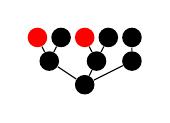
\begin{tikzpicture}[scale=.2]
\node[circle, scale=0.75, fill] (tid0) at (3.75,1.5){};
\node[circle, scale=0.75, fill] (tid1) at (1.5,3){};
\node[circle, scale=0.75, fill, red] (tid4) at (0.75,4.5){};
\node[circle, scale=0.75, fill] (tid5) at (2.25,4.5){};
\draw[](tid1) -- (tid4);
\draw[](tid1) -- (tid5);
\node[circle, scale=0.75, fill] (tid2) at (4.5,3){};
\node[circle, scale=0.75, fill, red] (tid6) at (3.75,4.5){};
\node[circle, scale=0.75, fill] (tid7) at (5.25,4.5){};
\draw[](tid2) -- (tid6);
\draw[](tid2) -- (tid7);
\node[circle, scale=0.75, fill] (tid3) at (6.75,3){};
\node[circle, scale=0.75, fill] (tid8) at (6.75,4.5){};
\draw[](tid3) -- (tid8);
\draw[](tid0) -- (tid1);
\draw[](tid0) -- (tid2);
\draw[](tid0) -- (tid3);
\end{tikzpicture}
\nodepart{three}
\footnotesize{5.625}
\nodepart{four}
\footnotesize{$67\:33$}
};
 & 
\node[draw=black, rectangle split,  rectangle split parts=3] (sn0x21e3370){
\footnotesize{0.125}
\nodepart{two}
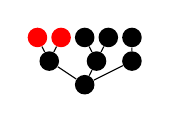
\begin{tikzpicture}[scale=.2]
\node[circle, scale=0.75, fill] (tid0) at (3.75,1.5){};
\node[circle, scale=0.75, fill] (tid1) at (1.5,3){};
\node[circle, scale=0.75, fill, red] (tid4) at (0.75,4.5){};
\node[circle, scale=0.75, fill, red] (tid5) at (2.25,4.5){};
\draw[](tid1) -- (tid4);
\draw[](tid1) -- (tid5);
\node[circle, scale=0.75, fill] (tid2) at (4.5,3){};
\node[circle, scale=0.75, fill] (tid6) at (3.75,4.5){};
\node[circle, scale=0.75, fill] (tid7) at (5.25,4.5){};
\draw[](tid2) -- (tid6);
\draw[](tid2) -- (tid7);
\node[circle, scale=0.75, fill] (tid3) at (6.75,3){};
\node[circle, scale=0.75, fill] (tid8) at (6.75,4.5){};
\draw[](tid3) -- (tid8);
\draw[](tid0) -- (tid1);
\draw[](tid0) -- (tid2);
\draw[](tid0) -- (tid3);
\end{tikzpicture}
\nodepart{three}
\footnotesize{5.625}
\nodepart{four}
\footnotesize{$67\:33$}
};
 & 
\node[draw=black, rectangle split,  rectangle split parts=3] (sn0x21e31c0){
\footnotesize{0.125}
\nodepart{two}
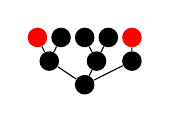
\begin{tikzpicture}[scale=.2]
\node[circle, scale=0.75, fill] (tid0) at (3.75,1.5){};
\node[circle, scale=0.75, fill] (tid1) at (1.5,3){};
\node[circle, scale=0.75, fill, red] (tid4) at (0.75,4.5){};
\node[circle, scale=0.75, fill] (tid5) at (2.25,4.5){};
\draw[](tid1) -- (tid4);
\draw[](tid1) -- (tid5);
\node[circle, scale=0.75, fill] (tid2) at (4.5,3){};
\node[circle, scale=0.75, fill] (tid6) at (3.75,4.5){};
\node[circle, scale=0.75, fill] (tid7) at (5.25,4.5){};
\draw[](tid2) -- (tid6);
\draw[](tid2) -- (tid7);
\node[circle, scale=0.75, fill] (tid3) at (6.75,3){};
\node[circle, scale=0.75, fill, red] (tid8) at (6.75,4.5){};
\draw[](tid3) -- (tid8);
\draw[](tid0) -- (tid1);
\draw[](tid0) -- (tid2);
\draw[](tid0) -- (tid3);
\end{tikzpicture}
\nodepart{three}
\footnotesize{5.625}
\nodepart{four}
\footnotesize{$33\:17\:17\:33$}
};
 & 
\node[draw=black, rectangle split,  rectangle split parts=3] (sn0x21e7540){
\footnotesize{0.25}
\nodepart{two}
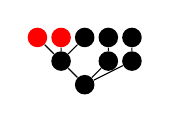
\begin{tikzpicture}[scale=.2]
\node[circle, scale=0.75, fill] (tid0) at (3.75,1.5){};
\node[circle, scale=0.75, fill] (tid1) at (2.25,3){};
\node[circle, scale=0.75, fill, red] (tid4) at (0.75,4.5){};
\node[circle, scale=0.75, fill, red] (tid5) at (2.25,4.5){};
\node[circle, scale=0.75, fill] (tid6) at (3.75,4.5){};
\draw[](tid1) -- (tid4);
\draw[](tid1) -- (tid5);
\draw[](tid1) -- (tid6);
\node[circle, scale=0.75, fill] (tid2) at (5.25,3){};
\node[circle, scale=0.75, fill] (tid7) at (5.25,4.5){};
\draw[](tid2) -- (tid7);
\node[circle, scale=0.75, fill] (tid3) at (6.75,3){};
\node[circle, scale=0.75, fill] (tid8) at (6.75,4.5){};
\draw[](tid3) -- (tid8);
\draw[](tid0) -- (tid1);
\draw[](tid0) -- (tid2);
\draw[](tid0) -- (tid3);
\end{tikzpicture}
\nodepart{three}
\footnotesize{5.625}
\nodepart{four}
\footnotesize{$67\:33$}
};
 & 
\node[draw=black, rectangle split,  rectangle split parts=3] (sn0x21e89a0){
\footnotesize{0.25}
\nodepart{two}
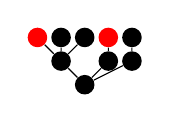
\begin{tikzpicture}[scale=.2]
\node[circle, scale=0.75, fill] (tid0) at (3.75,1.5){};
\node[circle, scale=0.75, fill] (tid1) at (2.25,3){};
\node[circle, scale=0.75, fill, red] (tid4) at (0.75,4.5){};
\node[circle, scale=0.75, fill] (tid5) at (2.25,4.5){};
\node[circle, scale=0.75, fill] (tid6) at (3.75,4.5){};
\draw[](tid1) -- (tid4);
\draw[](tid1) -- (tid5);
\draw[](tid1) -- (tid6);
\node[circle, scale=0.75, fill] (tid2) at (5.25,3){};
\node[circle, scale=0.75, fill, red] (tid7) at (5.25,4.5){};
\draw[](tid2) -- (tid7);
\node[circle, scale=0.75, fill] (tid3) at (6.75,3){};
\node[circle, scale=0.75, fill] (tid8) at (6.75,4.5){};
\draw[](tid3) -- (tid8);
\draw[](tid0) -- (tid1);
\draw[](tid0) -- (tid2);
\draw[](tid0) -- (tid3);
\end{tikzpicture}
\nodepart{three}
\footnotesize{5.625}
\nodepart{four}
\footnotesize{$33\:17\:33\:17$}
};
 & 
\\
};
\end{scope}
\begin{scope}[yshift=\leveltopIII cm]
\matrix (line3) [column sep=1cm] {
\node[draw=black, rectangle split,  rectangle split parts=3] (sn0x21e3fa0){
\footnotesize{0.541667}
\nodepart{two}
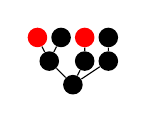
\begin{tikzpicture}[scale=.2]
\node[circle, scale=0.75, fill] (tid0) at (3,1.5){};
\node[circle, scale=0.75, fill] (tid1) at (1.5,3){};
\node[circle, scale=0.75, fill, red] (tid4) at (0.75,4.5){};
\node[circle, scale=0.75, fill] (tid5) at (2.25,4.5){};
\draw[](tid1) -- (tid4);
\draw[](tid1) -- (tid5);
\node[circle, scale=0.75, fill] (tid2) at (3.75,3){};
\node[circle, scale=0.75, fill, red] (tid6) at (3.75,4.5){};
\draw[](tid2) -- (tid6);
\node[circle, scale=0.75, fill] (tid3) at (5.25,3){};
\node[circle, scale=0.75, fill] (tid7) at (5.25,4.5){};
\draw[](tid3) -- (tid7);
\draw[](tid0) -- (tid1);
\draw[](tid0) -- (tid2);
\draw[](tid0) -- (tid3);
\end{tikzpicture}
\nodepart{three}
\footnotesize{5.125}
\nodepart{four}
\footnotesize{$50\:25\:25$}
};
 & 
\node[draw=black, rectangle split,  rectangle split parts=3] (sn0x21e7270){
\footnotesize{0.166667}
\nodepart{two}
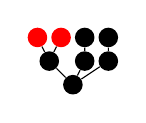
\begin{tikzpicture}[scale=.2]
\node[circle, scale=0.75, fill] (tid0) at (3,1.5){};
\node[circle, scale=0.75, fill] (tid1) at (1.5,3){};
\node[circle, scale=0.75, fill, red] (tid4) at (0.75,4.5){};
\node[circle, scale=0.75, fill, red] (tid5) at (2.25,4.5){};
\draw[](tid1) -- (tid4);
\draw[](tid1) -- (tid5);
\node[circle, scale=0.75, fill] (tid2) at (3.75,3){};
\node[circle, scale=0.75, fill] (tid6) at (3.75,4.5){};
\draw[](tid2) -- (tid6);
\node[circle, scale=0.75, fill] (tid3) at (5.25,3){};
\node[circle, scale=0.75, fill] (tid7) at (5.25,4.5){};
\draw[](tid3) -- (tid7);
\draw[](tid0) -- (tid1);
\draw[](tid0) -- (tid2);
\draw[](tid0) -- (tid3);
\end{tikzpicture}
\nodepart{three}
\footnotesize{5.125}
\nodepart{four}
\footnotesize{$1$}
};
 & 
\node[draw=black, rectangle split,  rectangle split parts=3] (sn0x21e4600){
\footnotesize{0.104167}
\nodepart{two}
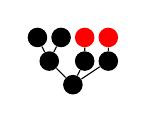
\begin{tikzpicture}[scale=.2]
\node[circle, scale=0.75, fill] (tid0) at (3,1.5){};
\node[circle, scale=0.75, fill] (tid1) at (1.5,3){};
\node[circle, scale=0.75, fill] (tid4) at (0.75,4.5){};
\node[circle, scale=0.75, fill] (tid5) at (2.25,4.5){};
\draw[](tid1) -- (tid4);
\draw[](tid1) -- (tid5);
\node[circle, scale=0.75, fill] (tid2) at (3.75,3){};
\node[circle, scale=0.75, fill, red] (tid6) at (3.75,4.5){};
\draw[](tid2) -- (tid6);
\node[circle, scale=0.75, fill] (tid3) at (5.25,3){};
\node[circle, scale=0.75, fill, red] (tid7) at (5.25,4.5){};
\draw[](tid3) -- (tid7);
\draw[](tid0) -- (tid1);
\draw[](tid0) -- (tid2);
\draw[](tid0) -- (tid3);
\end{tikzpicture}
\nodepart{three}
\footnotesize{5.125}
\nodepart{four}
\footnotesize{$1$}
};
 & 
\node[draw=black, rectangle split,  rectangle split parts=3] (sn0x21e79c0){
\footnotesize{0.0208333}
\nodepart{two}
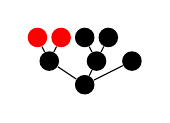
\begin{tikzpicture}[scale=.2]
\node[circle, scale=0.75, fill] (tid0) at (3.75,1.5){};
\node[circle, scale=0.75, fill] (tid1) at (1.5,3){};
\node[circle, scale=0.75, fill, red] (tid4) at (0.75,4.5){};
\node[circle, scale=0.75, fill, red] (tid5) at (2.25,4.5){};
\draw[](tid1) -- (tid4);
\draw[](tid1) -- (tid5);
\node[circle, scale=0.75, fill] (tid2) at (4.5,3){};
\node[circle, scale=0.75, fill] (tid6) at (3.75,4.5){};
\node[circle, scale=0.75, fill] (tid7) at (5.25,4.5){};
\draw[](tid2) -- (tid6);
\draw[](tid2) -- (tid7);
\node[circle, scale=0.75, fill] (tid3) at (6.75,3){};
\draw[](tid0) -- (tid1);
\draw[](tid0) -- (tid2);
\draw[](tid0) -- (tid3);
\end{tikzpicture}
\nodepart{three}
\footnotesize{5.125}
\nodepart{four}
\footnotesize{$1$}
};
 & 
\node[draw=black, rectangle split,  rectangle split parts=3] (sn0x21e6f50){
\footnotesize{0.0416667}
\nodepart{two}
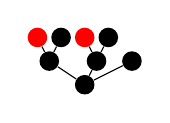
\begin{tikzpicture}[scale=.2]
\node[circle, scale=0.75, fill] (tid0) at (3.75,1.5){};
\node[circle, scale=0.75, fill] (tid1) at (1.5,3){};
\node[circle, scale=0.75, fill, red] (tid4) at (0.75,4.5){};
\node[circle, scale=0.75, fill] (tid5) at (2.25,4.5){};
\draw[](tid1) -- (tid4);
\draw[](tid1) -- (tid5);
\node[circle, scale=0.75, fill] (tid2) at (4.5,3){};
\node[circle, scale=0.75, fill, red] (tid6) at (3.75,4.5){};
\node[circle, scale=0.75, fill] (tid7) at (5.25,4.5){};
\draw[](tid2) -- (tid6);
\draw[](tid2) -- (tid7);
\node[circle, scale=0.75, fill] (tid3) at (6.75,3){};
\draw[](tid0) -- (tid1);
\draw[](tid0) -- (tid2);
\draw[](tid0) -- (tid3);
\end{tikzpicture}
\nodepart{three}
\footnotesize{5.125}
\nodepart{four}
\footnotesize{$50\:50$}
};
 & 
\node[draw=black, rectangle split,  rectangle split parts=3] (sn0x21e8c80){
\footnotesize{0.0833333}
\nodepart{two}
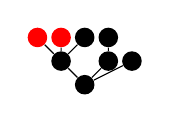
\begin{tikzpicture}[scale=.2]
\node[circle, scale=0.75, fill] (tid0) at (3.75,1.5){};
\node[circle, scale=0.75, fill] (tid1) at (2.25,3){};
\node[circle, scale=0.75, fill, red] (tid4) at (0.75,4.5){};
\node[circle, scale=0.75, fill, red] (tid5) at (2.25,4.5){};
\node[circle, scale=0.75, fill] (tid6) at (3.75,4.5){};
\draw[](tid1) -- (tid4);
\draw[](tid1) -- (tid5);
\draw[](tid1) -- (tid6);
\node[circle, scale=0.75, fill] (tid2) at (5.25,3){};
\node[circle, scale=0.75, fill] (tid7) at (5.25,4.5){};
\draw[](tid2) -- (tid7);
\node[circle, scale=0.75, fill] (tid3) at (6.75,3){};
\draw[](tid0) -- (tid1);
\draw[](tid0) -- (tid2);
\draw[](tid0) -- (tid3);
\end{tikzpicture}
\nodepart{three}
\footnotesize{5.125}
\nodepart{four}
\footnotesize{$50\:50$}
};
 & 
\node[draw=black, rectangle split,  rectangle split parts=3] (sn0x21e8870){
\footnotesize{0.0416667}
\nodepart{two}
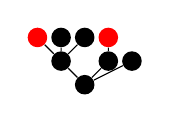
\begin{tikzpicture}[scale=.2]
\node[circle, scale=0.75, fill] (tid0) at (3.75,1.5){};
\node[circle, scale=0.75, fill] (tid1) at (2.25,3){};
\node[circle, scale=0.75, fill, red] (tid4) at (0.75,4.5){};
\node[circle, scale=0.75, fill] (tid5) at (2.25,4.5){};
\node[circle, scale=0.75, fill] (tid6) at (3.75,4.5){};
\draw[](tid1) -- (tid4);
\draw[](tid1) -- (tid5);
\draw[](tid1) -- (tid6);
\node[circle, scale=0.75, fill] (tid2) at (5.25,3){};
\node[circle, scale=0.75, fill, red] (tid7) at (5.25,4.5){};
\draw[](tid2) -- (tid7);
\node[circle, scale=0.75, fill] (tid3) at (6.75,3){};
\draw[](tid0) -- (tid1);
\draw[](tid0) -- (tid2);
\draw[](tid0) -- (tid3);
\end{tikzpicture}
\nodepart{three}
\footnotesize{5.125}
\nodepart{four}
\footnotesize{$50\:50$}
};
 & 
\\
};
\end{scope}
\begin{scope}[yshift=\leveltopIIII cm]
\matrix (line4) [column sep=1cm] {
\node[draw=black, rectangle split,  rectangle split parts=3] (sn0x21e4440){
\footnotesize{0.4375}
\nodepart{two}
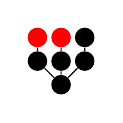
\begin{tikzpicture}[scale=.2]
\node[circle, scale=0.75, fill] (tid0) at (2.25,1.5){};
\node[circle, scale=0.75, fill] (tid1) at (0.75,3){};
\node[circle, scale=0.75, fill, red] (tid4) at (0.75,4.5){};
\draw[](tid1) -- (tid4);
\node[circle, scale=0.75, fill] (tid2) at (2.25,3){};
\node[circle, scale=0.75, fill, red] (tid5) at (2.25,4.5){};
\draw[](tid2) -- (tid5);
\node[circle, scale=0.75, fill] (tid3) at (3.75,3){};
\node[circle, scale=0.75, fill] (tid6) at (3.75,4.5){};
\draw[](tid3) -- (tid6);
\draw[](tid0) -- (tid1);
\draw[](tid0) -- (tid2);
\draw[](tid0) -- (tid3);
\end{tikzpicture}
\nodepart{three}
\footnotesize{4.625}
\nodepart{four}
\footnotesize{$1$}
};
 & 
\node[draw=black, rectangle split,  rectangle split parts=3] (sn0x21e48e0){
\footnotesize{0.197917}
\nodepart{two}
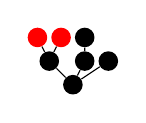
\begin{tikzpicture}[scale=.2]
\node[circle, scale=0.75, fill] (tid0) at (3,1.5){};
\node[circle, scale=0.75, fill] (tid1) at (1.5,3){};
\node[circle, scale=0.75, fill, red] (tid4) at (0.75,4.5){};
\node[circle, scale=0.75, fill, red] (tid5) at (2.25,4.5){};
\draw[](tid1) -- (tid4);
\draw[](tid1) -- (tid5);
\node[circle, scale=0.75, fill] (tid2) at (3.75,3){};
\node[circle, scale=0.75, fill] (tid6) at (3.75,4.5){};
\draw[](tid2) -- (tid6);
\node[circle, scale=0.75, fill] (tid3) at (5.25,3){};
\draw[](tid0) -- (tid1);
\draw[](tid0) -- (tid2);
\draw[](tid0) -- (tid3);
\end{tikzpicture}
\nodepart{three}
\footnotesize{4.625}
\nodepart{four}
\footnotesize{$1$}
};
 & 
\node[draw=black, rectangle split,  rectangle split parts=3] (sn0x21e49b0){
\footnotesize{0.34375}
\nodepart{two}
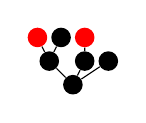
\begin{tikzpicture}[scale=.2]
\node[circle, scale=0.75, fill] (tid0) at (3,1.5){};
\node[circle, scale=0.75, fill] (tid1) at (1.5,3){};
\node[circle, scale=0.75, fill, red] (tid4) at (0.75,4.5){};
\node[circle, scale=0.75, fill] (tid5) at (2.25,4.5){};
\draw[](tid1) -- (tid4);
\draw[](tid1) -- (tid5);
\node[circle, scale=0.75, fill] (tid2) at (3.75,3){};
\node[circle, scale=0.75, fill, red] (tid6) at (3.75,4.5){};
\draw[](tid2) -- (tid6);
\node[circle, scale=0.75, fill] (tid3) at (5.25,3){};
\draw[](tid0) -- (tid1);
\draw[](tid0) -- (tid2);
\draw[](tid0) -- (tid3);
\end{tikzpicture}
\nodepart{three}
\footnotesize{4.625}
\nodepart{four}
\footnotesize{$50\:50$}
};
 & 
\node[draw=black, rectangle split,  rectangle split parts=3] (sn0x21e9950){
\footnotesize{0.0208333}
\nodepart{two}
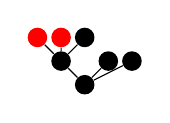
\begin{tikzpicture}[scale=.2]
\node[circle, scale=0.75, fill] (tid0) at (3.75,1.5){};
\node[circle, scale=0.75, fill] (tid1) at (2.25,3){};
\node[circle, scale=0.75, fill, red] (tid4) at (0.75,4.5){};
\node[circle, scale=0.75, fill, red] (tid5) at (2.25,4.5){};
\node[circle, scale=0.75, fill] (tid6) at (3.75,4.5){};
\draw[](tid1) -- (tid4);
\draw[](tid1) -- (tid5);
\draw[](tid1) -- (tid6);
\node[circle, scale=0.75, fill] (tid2) at (5.25,3){};
\node[circle, scale=0.75, fill] (tid3) at (6.75,3){};
\draw[](tid0) -- (tid1);
\draw[](tid0) -- (tid2);
\draw[](tid0) -- (tid3);
\end{tikzpicture}
\nodepart{three}
\footnotesize{4.625}
\nodepart{four}
\footnotesize{$1$}
};
 & 
\\
};
\end{scope}
\begin{scope}[yshift=\leveltopIIIII cm]
\matrix (line5) [column sep=1cm] {
\node[draw=black, rectangle split,  rectangle split parts=3] (sn0x21e5140){
\footnotesize{0.807292}
\nodepart{two}
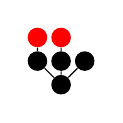
\begin{tikzpicture}[scale=.2]
\node[circle, scale=0.75, fill] (tid0) at (2.25,1.5){};
\node[circle, scale=0.75, fill] (tid1) at (0.75,3){};
\node[circle, scale=0.75, fill, red] (tid4) at (0.75,4.5){};
\draw[](tid1) -- (tid4);
\node[circle, scale=0.75, fill] (tid2) at (2.25,3){};
\node[circle, scale=0.75, fill, red] (tid5) at (2.25,4.5){};
\draw[](tid2) -- (tid5);
\node[circle, scale=0.75, fill] (tid3) at (3.75,3){};
\draw[](tid0) -- (tid1);
\draw[](tid0) -- (tid2);
\draw[](tid0) -- (tid3);
\end{tikzpicture}
\nodepart{three}
\footnotesize{4.125}
\nodepart{four}
\footnotesize{$1$}
};
 & 
\node[draw=black, rectangle split,  rectangle split parts=3] (sn0x21e5e90){
\footnotesize{0.192708}
\nodepart{two}
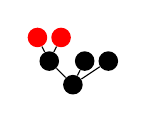
\begin{tikzpicture}[scale=.2]
\node[circle, scale=0.75, fill] (tid0) at (3,1.5){};
\node[circle, scale=0.75, fill] (tid1) at (1.5,3){};
\node[circle, scale=0.75, fill, red] (tid4) at (0.75,4.5){};
\node[circle, scale=0.75, fill, red] (tid5) at (2.25,4.5){};
\draw[](tid1) -- (tid4);
\draw[](tid1) -- (tid5);
\node[circle, scale=0.75, fill] (tid2) at (3.75,3){};
\node[circle, scale=0.75, fill] (tid3) at (5.25,3){};
\draw[](tid0) -- (tid1);
\draw[](tid0) -- (tid2);
\draw[](tid0) -- (tid3);
\end{tikzpicture}
\nodepart{three}
\footnotesize{4.125}
\nodepart{four}
\footnotesize{$1$}
};
 & 
\\
};
\end{scope}
\begin{scope}[yshift=\leveltopIIIIII cm]
\matrix (line6) [column sep=1cm] {
\node[draw=black, rectangle split,  rectangle split parts=3] (sn0x21e5300){
\footnotesize{1}
\nodepart{two}
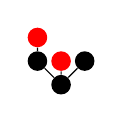
\begin{tikzpicture}[scale=.2]
\node[circle, scale=0.75, fill] (tid0) at (2.25,1.5){};
\node[circle, scale=0.75, fill] (tid1) at (0.75,3){};
\node[circle, scale=0.75, fill, red] (tid4) at (0.75,4.5){};
\draw[](tid1) -- (tid4);
\node[circle, scale=0.75, fill, red] (tid2) at (2.25,3){};
\node[circle, scale=0.75, fill] (tid3) at (3.75,3){};
\draw[](tid0) -- (tid1);
\draw[](tid0) -- (tid2);
\draw[](tid0) -- (tid3);
\end{tikzpicture}
\nodepart{three}
\footnotesize{3.625}
\nodepart{four}
\footnotesize{$50\:50$}
};
 & 
\\
};
\end{scope}
\begin{scope}[yshift=\leveltopIIIIIII cm]
\matrix (line7) [column sep=1cm] {
\node[draw=black, rectangle split,  rectangle split parts=3] (sn0x21e4eb0){
\footnotesize{0.5}
\nodepart{two}
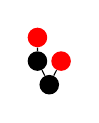
\begin{tikzpicture}[scale=.2]
\node[circle, scale=0.75, fill] (tid0) at (1.5,1.5){};
\node[circle, scale=0.75, fill] (tid1) at (0.75,3){};
\node[circle, scale=0.75, fill, red] (tid3) at (0.75,4.5){};
\draw[](tid1) -- (tid3);
\node[circle, scale=0.75, fill, red] (tid2) at (2.25,3){};
\draw[](tid0) -- (tid1);
\draw[](tid0) -- (tid2);
\end{tikzpicture}
\nodepart{three}
\footnotesize{3.25}
\nodepart{four}
\footnotesize{$50\:50$}
};
 & 
\node[draw=black, rectangle split,  rectangle split parts=3] (sn0x21e57b0){
\footnotesize{0.5}
\nodepart{two}
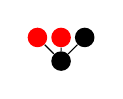
\begin{tikzpicture}[scale=.2]
\node[circle, scale=0.75, fill] (tid0) at (2.25,1.5){};
\node[circle, scale=0.75, fill, red] (tid1) at (0.75,3){};
\node[circle, scale=0.75, fill, red] (tid2) at (2.25,3){};
\node[circle, scale=0.75, fill] (tid3) at (3.75,3){};
\draw[](tid0) -- (tid1);
\draw[](tid0) -- (tid2);
\draw[](tid0) -- (tid3);
\end{tikzpicture}
\nodepart{three}
\footnotesize{3}
\nodepart{four}
\footnotesize{$1$}
};
 & 
\\
};
\end{scope}
\begin{scope}[yshift=\leveltopIIIIIIII cm]
\matrix (line8) [column sep=1cm] {
\node[draw=black, rectangle split,  rectangle split parts=3] (sn0x21e5880){
\footnotesize{0.25}
\nodepart{two}
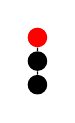
\begin{tikzpicture}[scale=.2]
\node[circle, scale=0.75, fill] (tid0) at (0.75,1.5){};
\node[circle, scale=0.75, fill] (tid1) at (0.75,3){};
\node[circle, scale=0.75, fill, red] (tid2) at (0.75,4.5){};
\draw[](tid1) -- (tid2);
\draw[](tid0) -- (tid1);
\end{tikzpicture}
\nodepart{three}
\footnotesize{3}
\nodepart{four}
\footnotesize{$1$}
};
 & 
\node[draw=black, rectangle split,  rectangle split parts=3] (sn0x21e5950){
\footnotesize{0.75}
\nodepart{two}

\begin{tikzpicture}[scale=.2]
\node[circle, scale=0.75, fill] (tid0) at (1.5,1.5){};
\node[circle, scale=0.75, fill, red] (tid1) at (0.75,3){};
\node[circle, scale=0.75, fill, red] (tid2) at (2.25,3){};
\draw[](tid0) -- (tid1);
\draw[](tid0) -- (tid2);
\end{tikzpicture}
\nodepart{three}
\footnotesize{2.5}
\nodepart{four}
\footnotesize{$1$}
};
 & 
\\
};
\end{scope}
\begin{scope}[yshift=\leveltopIIIIIIIII cm]
\matrix (line9) [column sep=1cm] {
\node[draw=black, rectangle split,  rectangle split parts=3] (sn0x21e5a20){
\footnotesize{1}
\nodepart{two}

\begin{tikzpicture}[scale=.2]
\node[circle, scale=0.75, fill] (tid0) at (0.75,1.5){};
\node[circle, scale=0.75, fill, red] (tid1) at (0.75,3){};
\draw[](tid0) -- (tid1);
\end{tikzpicture}
\nodepart{three}
\footnotesize{2}
\nodepart{four}
\footnotesize{$1$}
};
 & 
\\
};
\end{scope}
\begin{scope}[yshift=\leveltopIIIIIIIIII cm]
\matrix (line10) [column sep=1cm] {
\node[draw=black, rectangle split,  rectangle split parts=3] (sn0x21e5af0){
\footnotesize{1}
\nodepart{two}

\begin{tikzpicture}[scale=.2]
\node[circle, scale=0.75, fill, red] (tid0) at (0.75,1.5){};
\end{tikzpicture}
\nodepart{three}
\footnotesize{1}
\nodepart{four}
\footnotesize{$$}
};
 & 
\\
};
\end{scope}
\begin{scope}[yshift=\leveltopIIIIIIIIIII cm]
\matrix (line11) [column sep=1cm] {
\\
};
\end{scope}
\draw (sn0x21e1f80.south) -- (sn0x21e2ee0.north);
\draw (sn0x21e1f80.south) -- (sn0x21e3370.north);
\draw (sn0x21e1f80.south) -- (sn0x21e31c0.north);
\draw (sn0x21e1f80.south) -- (sn0x21e7540.north);
\draw (sn0x21e1f80.south) -- (sn0x21e89a0.north);
\draw (sn0x21e2ee0.south) -- (sn0x21e3fa0.north);
\draw (sn0x21e2ee0.south) -- (sn0x21e7270.north);
\draw (sn0x21e3370.south) -- (sn0x21e3fa0.north);
\draw (sn0x21e3370.south) -- (sn0x21e4600.north);
\draw (sn0x21e31c0.south) -- (sn0x21e4600.north);
\draw (sn0x21e31c0.south) -- (sn0x21e3fa0.north);
\draw (sn0x21e31c0.south) -- (sn0x21e79c0.north);
\draw (sn0x21e31c0.south) -- (sn0x21e6f50.north);
\draw (sn0x21e7540.south) -- (sn0x21e7270.north);
\draw (sn0x21e7540.south) -- (sn0x21e3fa0.north);
\draw (sn0x21e89a0.south) -- (sn0x21e3fa0.north);
\draw (sn0x21e89a0.south) -- (sn0x21e4600.north);
\draw (sn0x21e89a0.south) -- (sn0x21e8c80.north);
\draw (sn0x21e89a0.south) -- (sn0x21e8870.north);
\draw (sn0x21e3fa0.south) -- (sn0x21e4440.north);
\draw (sn0x21e3fa0.south) -- (sn0x21e48e0.north);
\draw (sn0x21e3fa0.south) -- (sn0x21e49b0.north);
\draw (sn0x21e7270.south) -- (sn0x21e4440.north);
\draw (sn0x21e4600.south) -- (sn0x21e49b0.north);
\draw (sn0x21e79c0.south) -- (sn0x21e49b0.north);
\draw (sn0x21e6f50.south) -- (sn0x21e49b0.north);
\draw (sn0x21e6f50.south) -- (sn0x21e48e0.north);
\draw (sn0x21e8c80.south) -- (sn0x21e48e0.north);
\draw (sn0x21e8c80.south) -- (sn0x21e49b0.north);
\draw (sn0x21e8870.south) -- (sn0x21e49b0.north);
\draw (sn0x21e8870.south) -- (sn0x21e9950.north);
\draw (sn0x21e4440.south) -- (sn0x21e5140.north);
\draw (sn0x21e48e0.south) -- (sn0x21e5140.north);
\draw (sn0x21e49b0.south) -- (sn0x21e5140.north);
\draw (sn0x21e49b0.south) -- (sn0x21e5e90.north);
\draw (sn0x21e9950.south) -- (sn0x21e5e90.north);
\draw (sn0x21e5140.south) -- (sn0x21e5300.north);
\draw (sn0x21e5e90.south) -- (sn0x21e5300.north);
\draw (sn0x21e5300.south) -- (sn0x21e4eb0.north);
\draw (sn0x21e5300.south) -- (sn0x21e57b0.north);
\draw (sn0x21e4eb0.south) -- (sn0x21e5880.north);
\draw (sn0x21e4eb0.south) -- (sn0x21e5950.north);
\draw (sn0x21e57b0.south) -- (sn0x21e5950.north);
\draw (sn0x21e5880.south) -- (sn0x21e5a20.north);
\draw (sn0x21e5950.south) -- (sn0x21e5a20.north);
\draw (sn0x21e5a20.south) -- (sn0x21e5af0.north);
\end{tikzpicture}

%%% Local Variables:
%%% TeX-master: "thesis/thesis.tex"
%%% End: 
\renewcommand{\leveltopI}{-15cm + \leveltop}
\renewcommand{\leveltopII}{-15cm + \leveltopI}
\renewcommand{\leveltopIII}{-15cm + \leveltopII}
\renewcommand{\leveltopIIII}{-15cm + \leveltopIII}
\renewcommand{\leveltopIIIII}{-15cm + \leveltopIIII}
\renewcommand{\leveltopIIIIII}{-15cm + \leveltopIIIII}
\renewcommand{\leveltopIIIIIII}{-15cm + \leveltopIIIIII}
\renewcommand{\leveltopIIIIIIII}{-15cm + \leveltopIIIIIII}
\renewcommand{\leveltopIIIIIIIII}{-15cm + \leveltopIIIIIIII}
\renewcommand{\leveltopIIIIIIIIII}{-15cm + \leveltopIIIIIIIII}
\begin{tikzpicture}[scale=.2, anchor=south]
\begin{scope}[yshift=\leveltopI cm]
\matrix (line1) [column sep=1cm] {
\node[draw=black, rectangle split,  rectangle split parts=3] (sn0x21e27a0){
\footnotesize{1}
\nodepart{two}
\begin{tikzpicture}[scale=.2]
\node[circle, scale=0.75, fill] (tid0) at (4.5,1.5){};
\node[circle, scale=0.75, fill] (tid1) at (2.25,3){};
\node[circle, scale=0.75, fill, red] (tid4) at (0.75,4.5){};
\node[circle, scale=0.75, fill] (tid5) at (2.25,4.5){};
\node[circle, scale=0.75, fill] (tid6) at (3.75,4.5){};
\draw[](tid1) -- (tid4);
\draw[](tid1) -- (tid5);
\draw[](tid1) -- (tid6);
\node[circle, scale=0.75, fill] (tid2) at (6,3){};
\node[circle, scale=0.75, fill] (tid7) at (5.25,4.5){};
\node[circle, scale=0.75, fill] (tid8) at (6.75,4.5){};
\draw[](tid2) -- (tid7);
\draw[](tid2) -- (tid8);
\node[circle, scale=0.75, fill] (tid3) at (8.25,3){};
\node[circle, scale=0.75, fill, red] (tid9) at (8.25,4.5){};
\draw[](tid3) -- (tid9);
\draw[](tid0) -- (tid1);
\draw[](tid0) -- (tid2);
\draw[](tid0) -- (tid3);
\end{tikzpicture}
\nodepart{three}
\footnotesize{6.125}
\nodepart{four}
\footnotesize{$50\:25\:25$}
};
 & 
\\
};
\end{scope}
\begin{scope}[yshift=\leveltopII cm]
\matrix (line2) [column sep=1cm] {
\node[draw=black, rectangle split,  rectangle split parts=3] (sn0x21e31c0){
\footnotesize{0.5}
\nodepart{two}
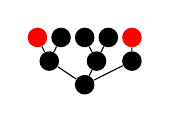
\begin{tikzpicture}[scale=.2]
\node[circle, scale=0.75, fill] (tid0) at (3.75,1.5){};
\node[circle, scale=0.75, fill] (tid1) at (1.5,3){};
\node[circle, scale=0.75, fill, red] (tid4) at (0.75,4.5){};
\node[circle, scale=0.75, fill] (tid5) at (2.25,4.5){};
\draw[](tid1) -- (tid4);
\draw[](tid1) -- (tid5);
\node[circle, scale=0.75, fill] (tid2) at (4.5,3){};
\node[circle, scale=0.75, fill] (tid6) at (3.75,4.5){};
\node[circle, scale=0.75, fill] (tid7) at (5.25,4.5){};
\draw[](tid2) -- (tid6);
\draw[](tid2) -- (tid7);
\node[circle, scale=0.75, fill] (tid3) at (6.75,3){};
\node[circle, scale=0.75, fill, red] (tid8) at (6.75,4.5){};
\draw[](tid3) -- (tid8);
\draw[](tid0) -- (tid1);
\draw[](tid0) -- (tid2);
\draw[](tid0) -- (tid3);
\end{tikzpicture}
\nodepart{three}
\footnotesize{5.625}
\nodepart{four}
\footnotesize{$17\:33\:17\:33$}
};
 & 
\node[draw=black, rectangle split,  rectangle split parts=3] (sn0x21e9040){
\footnotesize{0.25}
\nodepart{two}
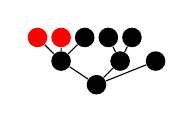
\begin{tikzpicture}[scale=.2]
\node[circle, scale=0.75, fill] (tid0) at (4.5,1.5){};
\node[circle, scale=0.75, fill] (tid1) at (2.25,3){};
\node[circle, scale=0.75, fill, red] (tid4) at (0.75,4.5){};
\node[circle, scale=0.75, fill, red] (tid5) at (2.25,4.5){};
\node[circle, scale=0.75, fill] (tid6) at (3.75,4.5){};
\draw[](tid1) -- (tid4);
\draw[](tid1) -- (tid5);
\draw[](tid1) -- (tid6);
\node[circle, scale=0.75, fill] (tid2) at (6,3){};
\node[circle, scale=0.75, fill] (tid7) at (5.25,4.5){};
\node[circle, scale=0.75, fill] (tid8) at (6.75,4.5){};
\draw[](tid2) -- (tid7);
\draw[](tid2) -- (tid8);
\node[circle, scale=0.75, fill] (tid3) at (8.25,3){};
\draw[](tid0) -- (tid1);
\draw[](tid0) -- (tid2);
\draw[](tid0) -- (tid3);
\end{tikzpicture}
\nodepart{three}
\footnotesize{5.625}
\nodepart{four}
\footnotesize{$33\:67$}
};
 & 
\node[draw=black, rectangle split,  rectangle split parts=3] (sn0x21ea6e0){
\footnotesize{0.25}
\nodepart{two}
\begin{tikzpicture}[scale=.2]
\node[circle, scale=0.75, fill] (tid0) at (4.5,1.5){};
\node[circle, scale=0.75, fill] (tid1) at (2.25,3){};
\node[circle, scale=0.75, fill, red] (tid4) at (0.75,4.5){};
\node[circle, scale=0.75, fill] (tid5) at (2.25,4.5){};
\node[circle, scale=0.75, fill] (tid6) at (3.75,4.5){};
\draw[](tid1) -- (tid4);
\draw[](tid1) -- (tid5);
\draw[](tid1) -- (tid6);
\node[circle, scale=0.75, fill] (tid2) at (6,3){};
\node[circle, scale=0.75, fill, red] (tid7) at (5.25,4.5){};
\node[circle, scale=0.75, fill] (tid8) at (6.75,4.5){};
\draw[](tid2) -- (tid7);
\draw[](tid2) -- (tid8);
\node[circle, scale=0.75, fill] (tid3) at (8.25,3){};
\draw[](tid0) -- (tid1);
\draw[](tid0) -- (tid2);
\draw[](tid0) -- (tid3);
\end{tikzpicture}
\nodepart{three}
\footnotesize{5.625}
\nodepart{four}
\footnotesize{$17\:33\:33\:17$}
};
 & 
\\
};
\end{scope}
\begin{scope}[yshift=\leveltopIII cm]
\matrix (line3) [column sep=1cm] {
\node[draw=black, rectangle split,  rectangle split parts=3] (sn0x21e4600){
\footnotesize{0.0833333}
\nodepart{two}
\begin{tikzpicture}[scale=.2]
\node[circle, scale=0.75, fill] (tid0) at (3,1.5){};
\node[circle, scale=0.75, fill] (tid1) at (1.5,3){};
\node[circle, scale=0.75, fill] (tid4) at (0.75,4.5){};
\node[circle, scale=0.75, fill] (tid5) at (2.25,4.5){};
\draw[](tid1) -- (tid4);
\draw[](tid1) -- (tid5);
\node[circle, scale=0.75, fill] (tid2) at (3.75,3){};
\node[circle, scale=0.75, fill, red] (tid6) at (3.75,4.5){};
\draw[](tid2) -- (tid6);
\node[circle, scale=0.75, fill] (tid3) at (5.25,3){};
\node[circle, scale=0.75, fill, red] (tid7) at (5.25,4.5){};
\draw[](tid3) -- (tid7);
\draw[](tid0) -- (tid1);
\draw[](tid0) -- (tid2);
\draw[](tid0) -- (tid3);
\end{tikzpicture}
\nodepart{three}
\footnotesize{5.125}
\nodepart{four}
\footnotesize{$1$}
};
 & 
\node[draw=black, rectangle split,  rectangle split parts=3] (sn0x21e3fa0){
\footnotesize{0.166667}
\nodepart{two}
\begin{tikzpicture}[scale=.2]
\node[circle, scale=0.75, fill] (tid0) at (3,1.5){};
\node[circle, scale=0.75, fill] (tid1) at (1.5,3){};
\node[circle, scale=0.75, fill, red] (tid4) at (0.75,4.5){};
\node[circle, scale=0.75, fill] (tid5) at (2.25,4.5){};
\draw[](tid1) -- (tid4);
\draw[](tid1) -- (tid5);
\node[circle, scale=0.75, fill] (tid2) at (3.75,3){};
\node[circle, scale=0.75, fill, red] (tid6) at (3.75,4.5){};
\draw[](tid2) -- (tid6);
\node[circle, scale=0.75, fill] (tid3) at (5.25,3){};
\node[circle, scale=0.75, fill] (tid7) at (5.25,4.5){};
\draw[](tid3) -- (tid7);
\draw[](tid0) -- (tid1);
\draw[](tid0) -- (tid2);
\draw[](tid0) -- (tid3);
\end{tikzpicture}
\nodepart{three}
\footnotesize{5.125}
\nodepart{four}
\footnotesize{$25\:50\:25$}
};
 & 
\node[draw=black, rectangle split,  rectangle split parts=3] (sn0x21e79c0){
\footnotesize{0.208333}
\nodepart{two}
\begin{tikzpicture}[scale=.2]
\node[circle, scale=0.75, fill] (tid0) at (3.75,1.5){};
\node[circle, scale=0.75, fill] (tid1) at (1.5,3){};
\node[circle, scale=0.75, fill, red] (tid4) at (0.75,4.5){};
\node[circle, scale=0.75, fill, red] (tid5) at (2.25,4.5){};
\draw[](tid1) -- (tid4);
\draw[](tid1) -- (tid5);
\node[circle, scale=0.75, fill] (tid2) at (4.5,3){};
\node[circle, scale=0.75, fill] (tid6) at (3.75,4.5){};
\node[circle, scale=0.75, fill] (tid7) at (5.25,4.5){};
\draw[](tid2) -- (tid6);
\draw[](tid2) -- (tid7);
\node[circle, scale=0.75, fill] (tid3) at (6.75,3){};
\draw[](tid0) -- (tid1);
\draw[](tid0) -- (tid2);
\draw[](tid0) -- (tid3);
\end{tikzpicture}
\nodepart{three}
\footnotesize{5.125}
\nodepart{four}
\footnotesize{$1$}
};
 & 
\node[draw=black, rectangle split,  rectangle split parts=3] (sn0x21e6f50){
\footnotesize{0.416667}
\nodepart{two}
\begin{tikzpicture}[scale=.2]
\node[circle, scale=0.75, fill] (tid0) at (3.75,1.5){};
\node[circle, scale=0.75, fill] (tid1) at (1.5,3){};
\node[circle, scale=0.75, fill, red] (tid4) at (0.75,4.5){};
\node[circle, scale=0.75, fill] (tid5) at (2.25,4.5){};
\draw[](tid1) -- (tid4);
\draw[](tid1) -- (tid5);
\node[circle, scale=0.75, fill] (tid2) at (4.5,3){};
\node[circle, scale=0.75, fill, red] (tid6) at (3.75,4.5){};
\node[circle, scale=0.75, fill] (tid7) at (5.25,4.5){};
\draw[](tid2) -- (tid6);
\draw[](tid2) -- (tid7);
\node[circle, scale=0.75, fill] (tid3) at (6.75,3){};
\draw[](tid0) -- (tid1);
\draw[](tid0) -- (tid2);
\draw[](tid0) -- (tid3);
\end{tikzpicture}
\nodepart{three}
\footnotesize{5.125}
\nodepart{four}
\footnotesize{$50\:50$}
};
 & 
\node[draw=black, rectangle split,  rectangle split parts=3] (sn0x21e8c80){
\footnotesize{0.0833333}
\nodepart{two}
\begin{tikzpicture}[scale=.2]
\node[circle, scale=0.75, fill] (tid0) at (3.75,1.5){};
\node[circle, scale=0.75, fill] (tid1) at (2.25,3){};
\node[circle, scale=0.75, fill, red] (tid4) at (0.75,4.5){};
\node[circle, scale=0.75, fill, red] (tid5) at (2.25,4.5){};
\node[circle, scale=0.75, fill] (tid6) at (3.75,4.5){};
\draw[](tid1) -- (tid4);
\draw[](tid1) -- (tid5);
\draw[](tid1) -- (tid6);
\node[circle, scale=0.75, fill] (tid2) at (5.25,3){};
\node[circle, scale=0.75, fill] (tid7) at (5.25,4.5){};
\draw[](tid2) -- (tid7);
\node[circle, scale=0.75, fill] (tid3) at (6.75,3){};
\draw[](tid0) -- (tid1);
\draw[](tid0) -- (tid2);
\draw[](tid0) -- (tid3);
\end{tikzpicture}
\nodepart{three}
\footnotesize{5.125}
\nodepart{four}
\footnotesize{$50\:50$}
};
 & 
\node[draw=black, rectangle split,  rectangle split parts=3] (sn0x21e8870){
\footnotesize{0.0416667}
\nodepart{two}
\begin{tikzpicture}[scale=.2]
\node[circle, scale=0.75, fill] (tid0) at (3.75,1.5){};
\node[circle, scale=0.75, fill] (tid1) at (2.25,3){};
\node[circle, scale=0.75, fill, red] (tid4) at (0.75,4.5){};
\node[circle, scale=0.75, fill] (tid5) at (2.25,4.5){};
\node[circle, scale=0.75, fill] (tid6) at (3.75,4.5){};
\draw[](tid1) -- (tid4);
\draw[](tid1) -- (tid5);
\draw[](tid1) -- (tid6);
\node[circle, scale=0.75, fill] (tid2) at (5.25,3){};
\node[circle, scale=0.75, fill, red] (tid7) at (5.25,4.5){};
\draw[](tid2) -- (tid7);
\node[circle, scale=0.75, fill] (tid3) at (6.75,3){};
\draw[](tid0) -- (tid1);
\draw[](tid0) -- (tid2);
\draw[](tid0) -- (tid3);
\end{tikzpicture}
\nodepart{three}
\footnotesize{5.125}
\nodepart{four}
\footnotesize{$50\:50$}
};
 & 
\\
};
\end{scope}
\begin{scope}[yshift=\leveltopIIII cm]
\matrix (line4) [column sep=1cm] {
\node[draw=black, rectangle split,  rectangle split parts=3] (sn0x21e49b0){
\footnotesize{0.604167}
\nodepart{two}
\begin{tikzpicture}[scale=.2]
\node[circle, scale=0.75, fill] (tid0) at (3,1.5){};
\node[circle, scale=0.75, fill] (tid1) at (1.5,3){};
\node[circle, scale=0.75, fill, red] (tid4) at (0.75,4.5){};
\node[circle, scale=0.75, fill] (tid5) at (2.25,4.5){};
\draw[](tid1) -- (tid4);
\draw[](tid1) -- (tid5);
\node[circle, scale=0.75, fill] (tid2) at (3.75,3){};
\node[circle, scale=0.75, fill, red] (tid6) at (3.75,4.5){};
\draw[](tid2) -- (tid6);
\node[circle, scale=0.75, fill] (tid3) at (5.25,3){};
\draw[](tid0) -- (tid1);
\draw[](tid0) -- (tid2);
\draw[](tid0) -- (tid3);
\end{tikzpicture}
\nodepart{three}
\footnotesize{4.625}
\nodepart{four}
\footnotesize{$50\:50$}
};
 & 
\node[draw=black, rectangle split,  rectangle split parts=3] (sn0x21e4440){
\footnotesize{0.0833333}
\nodepart{two}
\begin{tikzpicture}[scale=.2]
\node[circle, scale=0.75, fill] (tid0) at (2.25,1.5){};
\node[circle, scale=0.75, fill] (tid1) at (0.75,3){};
\node[circle, scale=0.75, fill, red] (tid4) at (0.75,4.5){};
\draw[](tid1) -- (tid4);
\node[circle, scale=0.75, fill] (tid2) at (2.25,3){};
\node[circle, scale=0.75, fill, red] (tid5) at (2.25,4.5){};
\draw[](tid2) -- (tid5);
\node[circle, scale=0.75, fill] (tid3) at (3.75,3){};
\node[circle, scale=0.75, fill] (tid6) at (3.75,4.5){};
\draw[](tid3) -- (tid6);
\draw[](tid0) -- (tid1);
\draw[](tid0) -- (tid2);
\draw[](tid0) -- (tid3);
\end{tikzpicture}
\nodepart{three}
\footnotesize{4.625}
\nodepart{four}
\footnotesize{$1$}
};
 & 
\node[draw=black, rectangle split,  rectangle split parts=3] (sn0x21e48e0){
\footnotesize{0.291667}
\nodepart{two}
\begin{tikzpicture}[scale=.2]
\node[circle, scale=0.75, fill] (tid0) at (3,1.5){};
\node[circle, scale=0.75, fill] (tid1) at (1.5,3){};
\node[circle, scale=0.75, fill, red] (tid4) at (0.75,4.5){};
\node[circle, scale=0.75, fill, red] (tid5) at (2.25,4.5){};
\draw[](tid1) -- (tid4);
\draw[](tid1) -- (tid5);
\node[circle, scale=0.75, fill] (tid2) at (3.75,3){};
\node[circle, scale=0.75, fill] (tid6) at (3.75,4.5){};
\draw[](tid2) -- (tid6);
\node[circle, scale=0.75, fill] (tid3) at (5.25,3){};
\draw[](tid0) -- (tid1);
\draw[](tid0) -- (tid2);
\draw[](tid0) -- (tid3);
\end{tikzpicture}
\nodepart{three}
\footnotesize{4.625}
\nodepart{four}
\footnotesize{$1$}
};
 & 
\node[draw=black, rectangle split,  rectangle split parts=3] (sn0x21e9950){
\footnotesize{0.0208333}
\nodepart{two}
\begin{tikzpicture}[scale=.2]
\node[circle, scale=0.75, fill] (tid0) at (3.75,1.5){};
\node[circle, scale=0.75, fill] (tid1) at (2.25,3){};
\node[circle, scale=0.75, fill, red] (tid4) at (0.75,4.5){};
\node[circle, scale=0.75, fill, red] (tid5) at (2.25,4.5){};
\node[circle, scale=0.75, fill] (tid6) at (3.75,4.5){};
\draw[](tid1) -- (tid4);
\draw[](tid1) -- (tid5);
\draw[](tid1) -- (tid6);
\node[circle, scale=0.75, fill] (tid2) at (5.25,3){};
\node[circle, scale=0.75, fill] (tid3) at (6.75,3){};
\draw[](tid0) -- (tid1);
\draw[](tid0) -- (tid2);
\draw[](tid0) -- (tid3);
\end{tikzpicture}
\nodepart{three}
\footnotesize{4.625}
\nodepart{four}
\footnotesize{$1$}
};
 & 
\\
};
\end{scope}
\begin{scope}[yshift=\leveltopIIIII cm]
\matrix (line5) [column sep=1cm] {
\node[draw=black, rectangle split,  rectangle split parts=3] (sn0x21e5140){
\footnotesize{0.677083}
\nodepart{two}
\begin{tikzpicture}[scale=.2]
\node[circle, scale=0.75, fill] (tid0) at (2.25,1.5){};
\node[circle, scale=0.75, fill] (tid1) at (0.75,3){};
\node[circle, scale=0.75, fill, red] (tid4) at (0.75,4.5){};
\draw[](tid1) -- (tid4);
\node[circle, scale=0.75, fill] (tid2) at (2.25,3){};
\node[circle, scale=0.75, fill, red] (tid5) at (2.25,4.5){};
\draw[](tid2) -- (tid5);
\node[circle, scale=0.75, fill] (tid3) at (3.75,3){};
\draw[](tid0) -- (tid1);
\draw[](tid0) -- (tid2);
\draw[](tid0) -- (tid3);
\end{tikzpicture}
\nodepart{three}
\footnotesize{4.125}
\nodepart{four}
\footnotesize{$1$}
};
 & 
\node[draw=black, rectangle split,  rectangle split parts=3] (sn0x21e5e90){
\footnotesize{0.322917}
\nodepart{two}
\begin{tikzpicture}[scale=.2]
\node[circle, scale=0.75, fill] (tid0) at (3,1.5){};
\node[circle, scale=0.75, fill] (tid1) at (1.5,3){};
\node[circle, scale=0.75, fill, red] (tid4) at (0.75,4.5){};
\node[circle, scale=0.75, fill, red] (tid5) at (2.25,4.5){};
\draw[](tid1) -- (tid4);
\draw[](tid1) -- (tid5);
\node[circle, scale=0.75, fill] (tid2) at (3.75,3){};
\node[circle, scale=0.75, fill] (tid3) at (5.25,3){};
\draw[](tid0) -- (tid1);
\draw[](tid0) -- (tid2);
\draw[](tid0) -- (tid3);
\end{tikzpicture}
\nodepart{three}
\footnotesize{4.125}
\nodepart{four}
\footnotesize{$1$}
};
 & 
\\
};
\end{scope}
\begin{scope}[yshift=\leveltopIIIIII cm]
\matrix (line6) [column sep=1cm] {
\node[draw=black, rectangle split,  rectangle split parts=3] (sn0x21e5300){
\footnotesize{1}
\nodepart{two}
\begin{tikzpicture}[scale=.2]
\node[circle, scale=0.75, fill] (tid0) at (2.25,1.5){};
\node[circle, scale=0.75, fill] (tid1) at (0.75,3){};
\node[circle, scale=0.75, fill, red] (tid4) at (0.75,4.5){};
\draw[](tid1) -- (tid4);
\node[circle, scale=0.75, fill, red] (tid2) at (2.25,3){};
\node[circle, scale=0.75, fill] (tid3) at (3.75,3){};
\draw[](tid0) -- (tid1);
\draw[](tid0) -- (tid2);
\draw[](tid0) -- (tid3);
\end{tikzpicture}
\nodepart{three}
\footnotesize{3.625}
\nodepart{four}
\footnotesize{$50\:50$}
};
 & 
\\
};
\end{scope}
\begin{scope}[yshift=\leveltopIIIIIII cm]
\matrix (line7) [column sep=1cm] {
\node[draw=black, rectangle split,  rectangle split parts=3] (sn0x21e4eb0){
\footnotesize{0.5}
\nodepart{two}
\begin{tikzpicture}[scale=.2]
\node[circle, scale=0.75, fill] (tid0) at (1.5,1.5){};
\node[circle, scale=0.75, fill] (tid1) at (0.75,3){};
\node[circle, scale=0.75, fill, red] (tid3) at (0.75,4.5){};
\draw[](tid1) -- (tid3);
\node[circle, scale=0.75, fill, red] (tid2) at (2.25,3){};
\draw[](tid0) -- (tid1);
\draw[](tid0) -- (tid2);
\end{tikzpicture}
\nodepart{three}
\footnotesize{3.25}
\nodepart{four}
\footnotesize{$50\:50$}
};
 & 
\node[draw=black, rectangle split,  rectangle split parts=3] (sn0x21e57b0){
\footnotesize{0.5}
\nodepart{two}
\begin{tikzpicture}[scale=.2]
\node[circle, scale=0.75, fill] (tid0) at (2.25,1.5){};
\node[circle, scale=0.75, fill, red] (tid1) at (0.75,3){};
\node[circle, scale=0.75, fill, red] (tid2) at (2.25,3){};
\node[circle, scale=0.75, fill] (tid3) at (3.75,3){};
\draw[](tid0) -- (tid1);
\draw[](tid0) -- (tid2);
\draw[](tid0) -- (tid3);
\end{tikzpicture}
\nodepart{three}
\footnotesize{3}
\nodepart{four}
\footnotesize{$1$}
};
 & 
\\
};
\end{scope}
\begin{scope}[yshift=\leveltopIIIIIIII cm]
\matrix (line8) [column sep=1cm] {
\node[draw=black, rectangle split,  rectangle split parts=3] (sn0x21e5880){
\footnotesize{0.25}
\nodepart{two}
\begin{tikzpicture}[scale=.2]
\node[circle, scale=0.75, fill] (tid0) at (0.75,1.5){};
\node[circle, scale=0.75, fill] (tid1) at (0.75,3){};
\node[circle, scale=0.75, fill, red] (tid2) at (0.75,4.5){};
\draw[](tid1) -- (tid2);
\draw[](tid0) -- (tid1);
\end{tikzpicture}
\nodepart{three}
\footnotesize{3}
\nodepart{four}
\footnotesize{$1$}
};
 & 
\node[draw=black, rectangle split,  rectangle split parts=3] (sn0x21e5950){
\footnotesize{0.75}
\nodepart{two}
\begin{tikzpicture}[scale=.2]
\node[circle, scale=0.75, fill] (tid0) at (1.5,1.5){};
\node[circle, scale=0.75, fill, red] (tid1) at (0.75,3){};
\node[circle, scale=0.75, fill, red] (tid2) at (2.25,3){};
\draw[](tid0) -- (tid1);
\draw[](tid0) -- (tid2);
\end{tikzpicture}
\nodepart{three}
\footnotesize{2.5}
\nodepart{four}
\footnotesize{$1$}
};
 & 
\\
};
\end{scope}
\begin{scope}[yshift=\leveltopIIIIIIIII cm]
\matrix (line9) [column sep=1cm] {
\node[draw=black, rectangle split,  rectangle split parts=3] (sn0x21e5a20){
\footnotesize{1}
\nodepart{two}
\begin{tikzpicture}[scale=.2]
\node[circle, scale=0.75, fill] (tid0) at (0.75,1.5){};
\node[circle, scale=0.75, fill, red] (tid1) at (0.75,3){};
\draw[](tid0) -- (tid1);
\end{tikzpicture}
\nodepart{three}
\footnotesize{2}
\nodepart{four}
\footnotesize{$1$}
};
 & 
\\
};
\end{scope}
\begin{scope}[yshift=\leveltopIIIIIIIIII cm]
\matrix (line10) [column sep=1cm] {
\node[draw=black, rectangle split,  rectangle split parts=3] (sn0x21e5af0){
\footnotesize{1}
\nodepart{two}
\begin{tikzpicture}[scale=.2]
\node[circle, scale=0.75, fill, red] (tid0) at (0.75,1.5){};
\end{tikzpicture}
\nodepart{three}
\footnotesize{1}
\nodepart{four}
\footnotesize{$$}
};
 & 
\\
};
\end{scope}
\begin{scope}[yshift=\leveltopIIIIIIIIIII cm]
\matrix (line11) [column sep=1cm] {
\\
};
\end{scope}
\draw (sn0x21e27a0.south) -- (sn0x21e31c0.north);
\draw (sn0x21e27a0.south) -- (sn0x21e9040.north);
\draw (sn0x21e27a0.south) -- (sn0x21ea6e0.north);
\draw (sn0x21e31c0.south) -- (sn0x21e4600.north);
\draw (sn0x21e31c0.south) -- (sn0x21e3fa0.north);
\draw (sn0x21e31c0.south) -- (sn0x21e79c0.north);
\draw (sn0x21e31c0.south) -- (sn0x21e6f50.north);
\draw (sn0x21e9040.south) -- (sn0x21e79c0.north);
\draw (sn0x21e9040.south) -- (sn0x21e6f50.north);
\draw (sn0x21ea6e0.south) -- (sn0x21e6f50.north);
\draw (sn0x21ea6e0.south) -- (sn0x21e79c0.north);
\draw (sn0x21ea6e0.south) -- (sn0x21e8c80.north);
\draw (sn0x21ea6e0.south) -- (sn0x21e8870.north);
\draw (sn0x21e4600.south) -- (sn0x21e49b0.north);
\draw (sn0x21e3fa0.south) -- (sn0x21e4440.north);
\draw (sn0x21e3fa0.south) -- (sn0x21e48e0.north);
\draw (sn0x21e3fa0.south) -- (sn0x21e49b0.north);
\draw (sn0x21e79c0.south) -- (sn0x21e49b0.north);
\draw (sn0x21e6f50.south) -- (sn0x21e49b0.north);
\draw (sn0x21e6f50.south) -- (sn0x21e48e0.north);
\draw (sn0x21e8c80.south) -- (sn0x21e48e0.north);
\draw (sn0x21e8c80.south) -- (sn0x21e49b0.north);
\draw (sn0x21e8870.south) -- (sn0x21e49b0.north);
\draw (sn0x21e8870.south) -- (sn0x21e9950.north);
\draw (sn0x21e49b0.south) -- (sn0x21e5140.north);
\draw (sn0x21e49b0.south) -- (sn0x21e5e90.north);
\draw (sn0x21e4440.south) -- (sn0x21e5140.north);
\draw (sn0x21e48e0.south) -- (sn0x21e5140.north);
\draw (sn0x21e9950.south) -- (sn0x21e5e90.north);
\draw (sn0x21e5140.south) -- (sn0x21e5300.north);
\draw (sn0x21e5e90.south) -- (sn0x21e5300.north);
\draw (sn0x21e5300.south) -- (sn0x21e4eb0.north);
\draw (sn0x21e5300.south) -- (sn0x21e57b0.north);
\draw (sn0x21e4eb0.south) -- (sn0x21e5880.north);
\draw (sn0x21e4eb0.south) -- (sn0x21e5950.north);
\draw (sn0x21e57b0.south) -- (sn0x21e5950.north);
\draw (sn0x21e5880.south) -- (sn0x21e5a20.north);
\draw (sn0x21e5950.south) -- (sn0x21e5a20.north);
\draw (sn0x21e5a20.south) -- (sn0x21e5af0.north);
\end{tikzpicture}

%%% Local Variables:
%%% TeX-master: "thesis/thesis.tex"
%%% End: 
\renewcommand{\leveltopI}{-15cm + \leveltop}
\renewcommand{\leveltopII}{-15cm + \leveltopI}
\renewcommand{\leveltopIII}{-15cm + \leveltopII}
\renewcommand{\leveltopIIII}{-15cm + \leveltopIII}
\renewcommand{\leveltopIIIII}{-15cm + \leveltopIIII}
\renewcommand{\leveltopIIIIII}{-15cm + \leveltopIIIII}
\renewcommand{\leveltopIIIIIII}{-15cm + \leveltopIIIIII}
\renewcommand{\leveltopIIIIIIII}{-15cm + \leveltopIIIIIII}
\renewcommand{\leveltopIIIIIIIII}{-15cm + \leveltopIIIIIIII}
\renewcommand{\leveltopIIIIIIIIII}{-15cm + \leveltopIIIIIIIII}
\begin{tikzpicture}[scale=.2, anchor=south]
\begin{scope}[yshift=\leveltopI cm]
\matrix (line1) [column sep=1cm] {
\node[draw=black, rectangle split,  rectangle split parts=3] (sn0x21e2bf0){
\footnotesize{1}
\nodepart{two}
\begin{tikzpicture}[scale=.2]
\node[circle, scale=0.75, fill] (tid0) at (4.5,1.5){};
\node[circle, scale=0.75, fill] (tid1) at (2.25,3){};
\node[circle, scale=0.75, fill] (tid4) at (0.75,4.5){};
\node[circle, scale=0.75, fill] (tid5) at (2.25,4.5){};
\node[circle, scale=0.75, fill] (tid6) at (3.75,4.5){};
\draw[](tid1) -- (tid4);
\draw[](tid1) -- (tid5);
\draw[](tid1) -- (tid6);
\node[circle, scale=0.75, fill] (tid2) at (6,3){};
\node[circle, scale=0.75, fill, red] (tid7) at (5.25,4.5){};
\node[circle, scale=0.75, fill, red] (tid8) at (6.75,4.5){};
\draw[](tid2) -- (tid7);
\draw[](tid2) -- (tid8);
\node[circle, scale=0.75, fill] (tid3) at (8.25,3){};
\node[circle, scale=0.75, fill] (tid9) at (8.25,4.5){};
\draw[](tid3) -- (tid9);
\draw[](tid0) -- (tid1);
\draw[](tid0) -- (tid2);
\draw[](tid0) -- (tid3);
\end{tikzpicture}
\nodepart{three}
\footnotesize{6.125}
\nodepart{four}
\footnotesize{$75\:25$}
};
 & 
\\
};
\end{scope}
\begin{scope}[yshift=\leveltopII cm]
\matrix (line2) [column sep=1cm] {
\node[draw=black, rectangle split,  rectangle split parts=3] (sn0x21e89a0){
\footnotesize{0.75}
\nodepart{two}
\begin{tikzpicture}[scale=.2]
\node[circle, scale=0.75, fill] (tid0) at (3.75,1.5){};
\node[circle, scale=0.75, fill] (tid1) at (2.25,3){};
\node[circle, scale=0.75, fill, red] (tid4) at (0.75,4.5){};
\node[circle, scale=0.75, fill] (tid5) at (2.25,4.5){};
\node[circle, scale=0.75, fill] (tid6) at (3.75,4.5){};
\draw[](tid1) -- (tid4);
\draw[](tid1) -- (tid5);
\draw[](tid1) -- (tid6);
\node[circle, scale=0.75, fill] (tid2) at (5.25,3){};
\node[circle, scale=0.75, fill, red] (tid7) at (5.25,4.5){};
\draw[](tid2) -- (tid7);
\node[circle, scale=0.75, fill] (tid3) at (6.75,3){};
\node[circle, scale=0.75, fill] (tid8) at (6.75,4.5){};
\draw[](tid3) -- (tid8);
\draw[](tid0) -- (tid1);
\draw[](tid0) -- (tid2);
\draw[](tid0) -- (tid3);
\end{tikzpicture}
\nodepart{three}
\footnotesize{5.625}
\nodepart{four}
\footnotesize{$33\:17\:33\:17$}
};
 & 
\node[draw=black, rectangle split,  rectangle split parts=3] (sn0x21ea350){
\footnotesize{0.25}
\nodepart{two}
\begin{tikzpicture}[scale=.2]
\node[circle, scale=0.75, fill] (tid0) at (3.75,1.5){};
\node[circle, scale=0.75, fill] (tid1) at (2.25,3){};
\node[circle, scale=0.75, fill] (tid4) at (0.75,4.5){};
\node[circle, scale=0.75, fill] (tid5) at (2.25,4.5){};
\node[circle, scale=0.75, fill] (tid6) at (3.75,4.5){};
\draw[](tid1) -- (tid4);
\draw[](tid1) -- (tid5);
\draw[](tid1) -- (tid6);
\node[circle, scale=0.75, fill] (tid2) at (5.25,3){};
\node[circle, scale=0.75, fill, red] (tid7) at (5.25,4.5){};
\draw[](tid2) -- (tid7);
\node[circle, scale=0.75, fill] (tid3) at (6.75,3){};
\node[circle, scale=0.75, fill, red] (tid8) at (6.75,4.5){};
\draw[](tid3) -- (tid8);
\draw[](tid0) -- (tid1);
\draw[](tid0) -- (tid2);
\draw[](tid0) -- (tid3);
\end{tikzpicture}
\nodepart{three}
\footnotesize{5.625}
\nodepart{four}
\footnotesize{$1$}
};
 & 
\\
};
\end{scope}
\begin{scope}[yshift=\leveltopIII cm]
\matrix (line3) [column sep=1cm] {
\node[draw=black, rectangle split,  rectangle split parts=3] (sn0x21e3fa0){
\footnotesize{0.25}
\nodepart{two}
\begin{tikzpicture}[scale=.2]
\node[circle, scale=0.75, fill] (tid0) at (3,1.5){};
\node[circle, scale=0.75, fill] (tid1) at (1.5,3){};
\node[circle, scale=0.75, fill, red] (tid4) at (0.75,4.5){};
\node[circle, scale=0.75, fill] (tid5) at (2.25,4.5){};
\draw[](tid1) -- (tid4);
\draw[](tid1) -- (tid5);
\node[circle, scale=0.75, fill] (tid2) at (3.75,3){};
\node[circle, scale=0.75, fill, red] (tid6) at (3.75,4.5){};
\draw[](tid2) -- (tid6);
\node[circle, scale=0.75, fill] (tid3) at (5.25,3){};
\node[circle, scale=0.75, fill] (tid7) at (5.25,4.5){};
\draw[](tid3) -- (tid7);
\draw[](tid0) -- (tid1);
\draw[](tid0) -- (tid2);
\draw[](tid0) -- (tid3);
\end{tikzpicture}
\nodepart{three}
\footnotesize{5.125}
\nodepart{four}
\footnotesize{$50\:25\:25$}
};
 & 
\node[draw=black, rectangle split,  rectangle split parts=3] (sn0x21e4600){
\footnotesize{0.125}
\nodepart{two}
\begin{tikzpicture}[scale=.2]
\node[circle, scale=0.75, fill] (tid0) at (3,1.5){};
\node[circle, scale=0.75, fill] (tid1) at (1.5,3){};
\node[circle, scale=0.75, fill] (tid4) at (0.75,4.5){};
\node[circle, scale=0.75, fill] (tid5) at (2.25,4.5){};
\draw[](tid1) -- (tid4);
\draw[](tid1) -- (tid5);
\node[circle, scale=0.75, fill] (tid2) at (3.75,3){};
\node[circle, scale=0.75, fill, red] (tid6) at (3.75,4.5){};
\draw[](tid2) -- (tid6);
\node[circle, scale=0.75, fill] (tid3) at (5.25,3){};
\node[circle, scale=0.75, fill, red] (tid7) at (5.25,4.5){};
\draw[](tid3) -- (tid7);
\draw[](tid0) -- (tid1);
\draw[](tid0) -- (tid2);
\draw[](tid0) -- (tid3);
\end{tikzpicture}
\nodepart{three}
\footnotesize{5.125}
\nodepart{four}
\footnotesize{$1$}
};
 & 
\node[draw=black, rectangle split,  rectangle split parts=3] (sn0x21e8c80){
\footnotesize{0.25}
\nodepart{two}
\begin{tikzpicture}[scale=.2]
\node[circle, scale=0.75, fill] (tid0) at (3.75,1.5){};
\node[circle, scale=0.75, fill] (tid1) at (2.25,3){};
\node[circle, scale=0.75, fill, red] (tid4) at (0.75,4.5){};
\node[circle, scale=0.75, fill, red] (tid5) at (2.25,4.5){};
\node[circle, scale=0.75, fill] (tid6) at (3.75,4.5){};
\draw[](tid1) -- (tid4);
\draw[](tid1) -- (tid5);
\draw[](tid1) -- (tid6);
\node[circle, scale=0.75, fill] (tid2) at (5.25,3){};
\node[circle, scale=0.75, fill] (tid7) at (5.25,4.5){};
\draw[](tid2) -- (tid7);
\node[circle, scale=0.75, fill] (tid3) at (6.75,3){};
\draw[](tid0) -- (tid1);
\draw[](tid0) -- (tid2);
\draw[](tid0) -- (tid3);
\end{tikzpicture}
\nodepart{three}
\footnotesize{5.125}
\nodepart{four}
\footnotesize{$50\:50$}
};
 & 
\node[draw=black, rectangle split,  rectangle split parts=3] (sn0x21e8870){
\footnotesize{0.375}
\nodepart{two}
\begin{tikzpicture}[scale=.2]
\node[circle, scale=0.75, fill] (tid0) at (3.75,1.5){};
\node[circle, scale=0.75, fill] (tid1) at (2.25,3){};
\node[circle, scale=0.75, fill, red] (tid4) at (0.75,4.5){};
\node[circle, scale=0.75, fill] (tid5) at (2.25,4.5){};
\node[circle, scale=0.75, fill] (tid6) at (3.75,4.5){};
\draw[](tid1) -- (tid4);
\draw[](tid1) -- (tid5);
\draw[](tid1) -- (tid6);
\node[circle, scale=0.75, fill] (tid2) at (5.25,3){};
\node[circle, scale=0.75, fill, red] (tid7) at (5.25,4.5){};
\draw[](tid2) -- (tid7);
\node[circle, scale=0.75, fill] (tid3) at (6.75,3){};
\draw[](tid0) -- (tid1);
\draw[](tid0) -- (tid2);
\draw[](tid0) -- (tid3);
\end{tikzpicture}
\nodepart{three}
\footnotesize{5.125}
\nodepart{four}
\footnotesize{$50\:50$}
};
 & 
\\
};
\end{scope}
\begin{scope}[yshift=\leveltopIIII cm]
\matrix (line4) [column sep=1cm] {
\node[draw=black, rectangle split,  rectangle split parts=3] (sn0x21e4440){
\footnotesize{0.125}
\nodepart{two}
\begin{tikzpicture}[scale=.2]
\node[circle, scale=0.75, fill] (tid0) at (2.25,1.5){};
\node[circle, scale=0.75, fill] (tid1) at (0.75,3){};
\node[circle, scale=0.75, fill, red] (tid4) at (0.75,4.5){};
\draw[](tid1) -- (tid4);
\node[circle, scale=0.75, fill] (tid2) at (2.25,3){};
\node[circle, scale=0.75, fill, red] (tid5) at (2.25,4.5){};
\draw[](tid2) -- (tid5);
\node[circle, scale=0.75, fill] (tid3) at (3.75,3){};
\node[circle, scale=0.75, fill] (tid6) at (3.75,4.5){};
\draw[](tid3) -- (tid6);
\draw[](tid0) -- (tid1);
\draw[](tid0) -- (tid2);
\draw[](tid0) -- (tid3);
\end{tikzpicture}
\nodepart{three}
\footnotesize{4.625}
\nodepart{four}
\footnotesize{$1$}
};
 & 
\node[draw=black, rectangle split,  rectangle split parts=3] (sn0x21e48e0){
\footnotesize{0.1875}
\nodepart{two}
\begin{tikzpicture}[scale=.2]
\node[circle, scale=0.75, fill] (tid0) at (3,1.5){};
\node[circle, scale=0.75, fill] (tid1) at (1.5,3){};
\node[circle, scale=0.75, fill, red] (tid4) at (0.75,4.5){};
\node[circle, scale=0.75, fill, red] (tid5) at (2.25,4.5){};
\draw[](tid1) -- (tid4);
\draw[](tid1) -- (tid5);
\node[circle, scale=0.75, fill] (tid2) at (3.75,3){};
\node[circle, scale=0.75, fill] (tid6) at (3.75,4.5){};
\draw[](tid2) -- (tid6);
\node[circle, scale=0.75, fill] (tid3) at (5.25,3){};
\draw[](tid0) -- (tid1);
\draw[](tid0) -- (tid2);
\draw[](tid0) -- (tid3);
\end{tikzpicture}
\nodepart{three}
\footnotesize{4.625}
\nodepart{four}
\footnotesize{$1$}
};
 & 
\node[draw=black, rectangle split,  rectangle split parts=3] (sn0x21e49b0){
\footnotesize{0.5}
\nodepart{two}
\begin{tikzpicture}[scale=.2]
\node[circle, scale=0.75, fill] (tid0) at (3,1.5){};
\node[circle, scale=0.75, fill] (tid1) at (1.5,3){};
\node[circle, scale=0.75, fill, red] (tid4) at (0.75,4.5){};
\node[circle, scale=0.75, fill] (tid5) at (2.25,4.5){};
\draw[](tid1) -- (tid4);
\draw[](tid1) -- (tid5);
\node[circle, scale=0.75, fill] (tid2) at (3.75,3){};
\node[circle, scale=0.75, fill, red] (tid6) at (3.75,4.5){};
\draw[](tid2) -- (tid6);
\node[circle, scale=0.75, fill] (tid3) at (5.25,3){};
\draw[](tid0) -- (tid1);
\draw[](tid0) -- (tid2);
\draw[](tid0) -- (tid3);
\end{tikzpicture}
\nodepart{three}
\footnotesize{4.625}
\nodepart{four}
\footnotesize{$50\:50$}
};
 & 
\node[draw=black, rectangle split,  rectangle split parts=3] (sn0x21e9950){
\footnotesize{0.1875}
\nodepart{two}
\begin{tikzpicture}[scale=.2]
\node[circle, scale=0.75, fill] (tid0) at (3.75,1.5){};
\node[circle, scale=0.75, fill] (tid1) at (2.25,3){};
\node[circle, scale=0.75, fill, red] (tid4) at (0.75,4.5){};
\node[circle, scale=0.75, fill, red] (tid5) at (2.25,4.5){};
\node[circle, scale=0.75, fill] (tid6) at (3.75,4.5){};
\draw[](tid1) -- (tid4);
\draw[](tid1) -- (tid5);
\draw[](tid1) -- (tid6);
\node[circle, scale=0.75, fill] (tid2) at (5.25,3){};
\node[circle, scale=0.75, fill] (tid3) at (6.75,3){};
\draw[](tid0) -- (tid1);
\draw[](tid0) -- (tid2);
\draw[](tid0) -- (tid3);
\end{tikzpicture}
\nodepart{three}
\footnotesize{4.625}
\nodepart{four}
\footnotesize{$1$}
};
 & 
\\
};
\end{scope}
\begin{scope}[yshift=\leveltopIIIII cm]
\matrix (line5) [column sep=1cm] {
\node[draw=black, rectangle split,  rectangle split parts=3] (sn0x21e5140){
\footnotesize{0.5625}
\nodepart{two}
\begin{tikzpicture}[scale=.2]
\node[circle, scale=0.75, fill] (tid0) at (2.25,1.5){};
\node[circle, scale=0.75, fill] (tid1) at (0.75,3){};
\node[circle, scale=0.75, fill, red] (tid4) at (0.75,4.5){};
\draw[](tid1) -- (tid4);
\node[circle, scale=0.75, fill] (tid2) at (2.25,3){};
\node[circle, scale=0.75, fill, red] (tid5) at (2.25,4.5){};
\draw[](tid2) -- (tid5);
\node[circle, scale=0.75, fill] (tid3) at (3.75,3){};
\draw[](tid0) -- (tid1);
\draw[](tid0) -- (tid2);
\draw[](tid0) -- (tid3);
\end{tikzpicture}
\nodepart{three}
\footnotesize{4.125}
\nodepart{four}
\footnotesize{$1$}
};
 & 
\node[draw=black, rectangle split,  rectangle split parts=3] (sn0x21e5e90){
\footnotesize{0.4375}
\nodepart{two}
\begin{tikzpicture}[scale=.2]
\node[circle, scale=0.75, fill] (tid0) at (3,1.5){};
\node[circle, scale=0.75, fill] (tid1) at (1.5,3){};
\node[circle, scale=0.75, fill, red] (tid4) at (0.75,4.5){};
\node[circle, scale=0.75, fill, red] (tid5) at (2.25,4.5){};
\draw[](tid1) -- (tid4);
\draw[](tid1) -- (tid5);
\node[circle, scale=0.75, fill] (tid2) at (3.75,3){};
\node[circle, scale=0.75, fill] (tid3) at (5.25,3){};
\draw[](tid0) -- (tid1);
\draw[](tid0) -- (tid2);
\draw[](tid0) -- (tid3);
\end{tikzpicture}
\nodepart{three}
\footnotesize{4.125}
\nodepart{four}
\footnotesize{$1$}
};
 & 
\\
};
\end{scope}
\begin{scope}[yshift=\leveltopIIIIII cm]
\matrix (line6) [column sep=1cm] {
\node[draw=black, rectangle split,  rectangle split parts=3] (sn0x21e5300){
\footnotesize{1}
\nodepart{two}
\begin{tikzpicture}[scale=.2]
\node[circle, scale=0.75, fill] (tid0) at (2.25,1.5){};
\node[circle, scale=0.75, fill] (tid1) at (0.75,3){};
\node[circle, scale=0.75, fill, red] (tid4) at (0.75,4.5){};
\draw[](tid1) -- (tid4);
\node[circle, scale=0.75, fill, red] (tid2) at (2.25,3){};
\node[circle, scale=0.75, fill] (tid3) at (3.75,3){};
\draw[](tid0) -- (tid1);
\draw[](tid0) -- (tid2);
\draw[](tid0) -- (tid3);
\end{tikzpicture}
\nodepart{three}
\footnotesize{3.625}
\nodepart{four}
\footnotesize{$50\:50$}
};
 & 
\\
};
\end{scope}
\begin{scope}[yshift=\leveltopIIIIIII cm]
\matrix (line7) [column sep=1cm] {
\node[draw=black, rectangle split,  rectangle split parts=3] (sn0x21e4eb0){
\footnotesize{0.5}
\nodepart{two}
\begin{tikzpicture}[scale=.2]
\node[circle, scale=0.75, fill] (tid0) at (1.5,1.5){};
\node[circle, scale=0.75, fill] (tid1) at (0.75,3){};
\node[circle, scale=0.75, fill, red] (tid3) at (0.75,4.5){};
\draw[](tid1) -- (tid3);
\node[circle, scale=0.75, fill, red] (tid2) at (2.25,3){};
\draw[](tid0) -- (tid1);
\draw[](tid0) -- (tid2);
\end{tikzpicture}
\nodepart{three}
\footnotesize{3.25}
\nodepart{four}
\footnotesize{$50\:50$}
};
 & 
\node[draw=black, rectangle split,  rectangle split parts=3] (sn0x21e57b0){
\footnotesize{0.5}
\nodepart{two}
\begin{tikzpicture}[scale=.2]
\node[circle, scale=0.75, fill] (tid0) at (2.25,1.5){};
\node[circle, scale=0.75, fill, red] (tid1) at (0.75,3){};
\node[circle, scale=0.75, fill, red] (tid2) at (2.25,3){};
\node[circle, scale=0.75, fill] (tid3) at (3.75,3){};
\draw[](tid0) -- (tid1);
\draw[](tid0) -- (tid2);
\draw[](tid0) -- (tid3);
\end{tikzpicture}
\nodepart{three}
\footnotesize{3}
\nodepart{four}
\footnotesize{$1$}
};
 & 
\\
};
\end{scope}
\begin{scope}[yshift=\leveltopIIIIIIII cm]
\matrix (line8) [column sep=1cm] {
\node[draw=black, rectangle split,  rectangle split parts=3] (sn0x21e5880){
\footnotesize{0.25}
\nodepart{two}
\begin{tikzpicture}[scale=.2]
\node[circle, scale=0.75, fill] (tid0) at (0.75,1.5){};
\node[circle, scale=0.75, fill] (tid1) at (0.75,3){};
\node[circle, scale=0.75, fill, red] (tid2) at (0.75,4.5){};
\draw[](tid1) -- (tid2);
\draw[](tid0) -- (tid1);
\end{tikzpicture}
\nodepart{three}
\footnotesize{3}
\nodepart{four}
\footnotesize{$1$}
};
 & 
\node[draw=black, rectangle split,  rectangle split parts=3] (sn0x21e5950){
\footnotesize{0.75}
\nodepart{two}
\begin{tikzpicture}[scale=.2]
\node[circle, scale=0.75, fill] (tid0) at (1.5,1.5){};
\node[circle, scale=0.75, fill, red] (tid1) at (0.75,3){};
\node[circle, scale=0.75, fill, red] (tid2) at (2.25,3){};
\draw[](tid0) -- (tid1);
\draw[](tid0) -- (tid2);
\end{tikzpicture}
\nodepart{three}
\footnotesize{2.5}
\nodepart{four}
\footnotesize{$1$}
};
 & 
\\
};
\end{scope}
\begin{scope}[yshift=\leveltopIIIIIIIII cm]
\matrix (line9) [column sep=1cm] {
\node[draw=black, rectangle split,  rectangle split parts=3] (sn0x21e5a20){
\footnotesize{1}
\nodepart{two}
\begin{tikzpicture}[scale=.2]
\node[circle, scale=0.75, fill] (tid0) at (0.75,1.5){};
\node[circle, scale=0.75, fill, red] (tid1) at (0.75,3){};
\draw[](tid0) -- (tid1);
\end{tikzpicture}
\nodepart{three}
\footnotesize{2}
\nodepart{four}
\footnotesize{$1$}
};
 & 
\\
};
\end{scope}
\begin{scope}[yshift=\leveltopIIIIIIIIII cm]
\matrix (line10) [column sep=1cm] {
\node[draw=black, rectangle split,  rectangle split parts=3] (sn0x21e5af0){
\footnotesize{1}
\nodepart{two}
\begin{tikzpicture}[scale=.2]
\node[circle, scale=0.75, fill, red] (tid0) at (0.75,1.5){};
\end{tikzpicture}
\nodepart{three}
\footnotesize{1}
\nodepart{four}
\footnotesize{$$}
};
 & 
\\
};
\end{scope}
\begin{scope}[yshift=\leveltopIIIIIIIIIII cm]
\matrix (line11) [column sep=1cm] {
\\
};
\end{scope}
\draw (sn0x21e2bf0.south) -- (sn0x21e89a0.north);
\draw (sn0x21e2bf0.south) -- (sn0x21ea350.north);
\draw (sn0x21e89a0.south) -- (sn0x21e3fa0.north);
\draw (sn0x21e89a0.south) -- (sn0x21e4600.north);
\draw (sn0x21e89a0.south) -- (sn0x21e8c80.north);
\draw (sn0x21e89a0.south) -- (sn0x21e8870.north);
\draw (sn0x21ea350.south) -- (sn0x21e8870.north);
\draw (sn0x21e3fa0.south) -- (sn0x21e4440.north);
\draw (sn0x21e3fa0.south) -- (sn0x21e48e0.north);
\draw (sn0x21e3fa0.south) -- (sn0x21e49b0.north);
\draw (sn0x21e4600.south) -- (sn0x21e49b0.north);
\draw (sn0x21e8c80.south) -- (sn0x21e48e0.north);
\draw (sn0x21e8c80.south) -- (sn0x21e49b0.north);
\draw (sn0x21e8870.south) -- (sn0x21e49b0.north);
\draw (sn0x21e8870.south) -- (sn0x21e9950.north);
\draw (sn0x21e4440.south) -- (sn0x21e5140.north);
\draw (sn0x21e48e0.south) -- (sn0x21e5140.north);
\draw (sn0x21e49b0.south) -- (sn0x21e5140.north);
\draw (sn0x21e49b0.south) -- (sn0x21e5e90.north);
\draw (sn0x21e9950.south) -- (sn0x21e5e90.north);
\draw (sn0x21e5140.south) -- (sn0x21e5300.north);
\draw (sn0x21e5e90.south) -- (sn0x21e5300.north);
\draw (sn0x21e5300.south) -- (sn0x21e4eb0.north);
\draw (sn0x21e5300.south) -- (sn0x21e57b0.north);
\draw (sn0x21e4eb0.south) -- (sn0x21e5880.north);
\draw (sn0x21e4eb0.south) -- (sn0x21e5950.north);
\draw (sn0x21e57b0.south) -- (sn0x21e5950.north);
\draw (sn0x21e5880.south) -- (sn0x21e5a20.north);
\draw (sn0x21e5950.south) -- (sn0x21e5a20.north);
\draw (sn0x21e5a20.south) -- (sn0x21e5af0.north);
\end{tikzpicture}

%%% Local Variables:
%%% TeX-master: "thesis/thesis.tex"
%%% End: 
\renewcommand{\leveltopI}{-15cm + \leveltop}
\renewcommand{\leveltopII}{-15cm + \leveltopI}
\renewcommand{\leveltopIII}{-15cm + \leveltopII}
\renewcommand{\leveltopIIII}{-15cm + \leveltopIII}
\renewcommand{\leveltopIIIII}{-15cm + \leveltopIIII}
\renewcommand{\leveltopIIIIII}{-15cm + \leveltopIIIII}
\renewcommand{\leveltopIIIIIII}{-15cm + \leveltopIIIIII}
\renewcommand{\leveltopIIIIIIII}{-15cm + \leveltopIIIIIII}
\renewcommand{\leveltopIIIIIIIII}{-15cm + \leveltopIIIIIIII}
\renewcommand{\leveltopIIIIIIIIII}{-15cm + \leveltopIIIIIIIII}
\begin{tikzpicture}[scale=.2, anchor=south]
\begin{scope}[yshift=\leveltopI cm]
\matrix (line1) [column sep=1cm] {
\node[draw=black, rectangle split,  rectangle split parts=3] (sn0x21e2d10){
\footnotesize{1}
\nodepart{two}
\begin{tikzpicture}[scale=.2]
\node[circle, scale=0.75, fill] (tid0) at (4.5,1.5){};
\node[circle, scale=0.75, fill] (tid1) at (2.25,3){};
\node[circle, scale=0.75, fill] (tid4) at (0.75,4.5){};
\node[circle, scale=0.75, fill] (tid5) at (2.25,4.5){};
\node[circle, scale=0.75, fill] (tid6) at (3.75,4.5){};
\draw[](tid1) -- (tid4);
\draw[](tid1) -- (tid5);
\draw[](tid1) -- (tid6);
\node[circle, scale=0.75, fill] (tid2) at (6,3){};
\node[circle, scale=0.75, fill, red] (tid7) at (5.25,4.5){};
\node[circle, scale=0.75, fill] (tid8) at (6.75,4.5){};
\draw[](tid2) -- (tid7);
\draw[](tid2) -- (tid8);
\node[circle, scale=0.75, fill] (tid3) at (8.25,3){};
\node[circle, scale=0.75, fill, red] (tid9) at (8.25,4.5){};
\draw[](tid3) -- (tid9);
\draw[](tid0) -- (tid1);
\draw[](tid0) -- (tid2);
\draw[](tid0) -- (tid3);
\end{tikzpicture}
\nodepart{three}
\footnotesize{6.125}
\nodepart{four}
\footnotesize{$38\:12\:38\:12$}
};
 & 
\\
};
\end{scope}
\begin{scope}[yshift=\leveltopII cm]
\matrix (line2) [column sep=1cm] {
\node[draw=black, rectangle split,  rectangle split parts=3] (sn0x21e89a0){
\footnotesize{0.375}
\nodepart{two}
\begin{tikzpicture}[scale=.2]
\node[circle, scale=0.75, fill] (tid0) at (3.75,1.5){};
\node[circle, scale=0.75, fill] (tid1) at (2.25,3){};
\node[circle, scale=0.75, fill, red] (tid4) at (0.75,4.5){};
\node[circle, scale=0.75, fill] (tid5) at (2.25,4.5){};
\node[circle, scale=0.75, fill] (tid6) at (3.75,4.5){};
\draw[](tid1) -- (tid4);
\draw[](tid1) -- (tid5);
\draw[](tid1) -- (tid6);
\node[circle, scale=0.75, fill] (tid2) at (5.25,3){};
\node[circle, scale=0.75, fill, red] (tid7) at (5.25,4.5){};
\draw[](tid2) -- (tid7);
\node[circle, scale=0.75, fill] (tid3) at (6.75,3){};
\node[circle, scale=0.75, fill] (tid8) at (6.75,4.5){};
\draw[](tid3) -- (tid8);
\draw[](tid0) -- (tid1);
\draw[](tid0) -- (tid2);
\draw[](tid0) -- (tid3);
\end{tikzpicture}
\nodepart{three}
\footnotesize{5.625}
\nodepart{four}
\footnotesize{$33\:17\:33\:17$}
};
 & 
\node[draw=black, rectangle split,  rectangle split parts=3] (sn0x21ea350){
\footnotesize{0.125}
\nodepart{two}
\begin{tikzpicture}[scale=.2]
\node[circle, scale=0.75, fill] (tid0) at (3.75,1.5){};
\node[circle, scale=0.75, fill] (tid1) at (2.25,3){};
\node[circle, scale=0.75, fill] (tid4) at (0.75,4.5){};
\node[circle, scale=0.75, fill] (tid5) at (2.25,4.5){};
\node[circle, scale=0.75, fill] (tid6) at (3.75,4.5){};
\draw[](tid1) -- (tid4);
\draw[](tid1) -- (tid5);
\draw[](tid1) -- (tid6);
\node[circle, scale=0.75, fill] (tid2) at (5.25,3){};
\node[circle, scale=0.75, fill, red] (tid7) at (5.25,4.5){};
\draw[](tid2) -- (tid7);
\node[circle, scale=0.75, fill] (tid3) at (6.75,3){};
\node[circle, scale=0.75, fill, red] (tid8) at (6.75,4.5){};
\draw[](tid3) -- (tid8);
\draw[](tid0) -- (tid1);
\draw[](tid0) -- (tid2);
\draw[](tid0) -- (tid3);
\end{tikzpicture}
\nodepart{three}
\footnotesize{5.625}
\nodepart{four}
\footnotesize{$1$}
};
 & 
\node[draw=black, rectangle split,  rectangle split parts=3] (sn0x21ea6e0){
\footnotesize{0.375}
\nodepart{two}
\begin{tikzpicture}[scale=.2]
\node[circle, scale=0.75, fill] (tid0) at (4.5,1.5){};
\node[circle, scale=0.75, fill] (tid1) at (2.25,3){};
\node[circle, scale=0.75, fill, red] (tid4) at (0.75,4.5){};
\node[circle, scale=0.75, fill] (tid5) at (2.25,4.5){};
\node[circle, scale=0.75, fill] (tid6) at (3.75,4.5){};
\draw[](tid1) -- (tid4);
\draw[](tid1) -- (tid5);
\draw[](tid1) -- (tid6);
\node[circle, scale=0.75, fill] (tid2) at (6,3){};
\node[circle, scale=0.75, fill, red] (tid7) at (5.25,4.5){};
\node[circle, scale=0.75, fill] (tid8) at (6.75,4.5){};
\draw[](tid2) -- (tid7);
\draw[](tid2) -- (tid8);
\node[circle, scale=0.75, fill] (tid3) at (8.25,3){};
\draw[](tid0) -- (tid1);
\draw[](tid0) -- (tid2);
\draw[](tid0) -- (tid3);
\end{tikzpicture}
\nodepart{three}
\footnotesize{5.625}
\nodepart{four}
\footnotesize{$33\:17\:33\:17$}
};
 & 
\node[draw=black, rectangle split,  rectangle split parts=3] (sn0x21eaa90){
\footnotesize{0.125}
\nodepart{two}
\begin{tikzpicture}[scale=.2]
\node[circle, scale=0.75, fill] (tid0) at (4.5,1.5){};
\node[circle, scale=0.75, fill] (tid1) at (2.25,3){};
\node[circle, scale=0.75, fill] (tid4) at (0.75,4.5){};
\node[circle, scale=0.75, fill] (tid5) at (2.25,4.5){};
\node[circle, scale=0.75, fill] (tid6) at (3.75,4.5){};
\draw[](tid1) -- (tid4);
\draw[](tid1) -- (tid5);
\draw[](tid1) -- (tid6);
\node[circle, scale=0.75, fill] (tid2) at (6,3){};
\node[circle, scale=0.75, fill, red] (tid7) at (5.25,4.5){};
\node[circle, scale=0.75, fill, red] (tid8) at (6.75,4.5){};
\draw[](tid2) -- (tid7);
\draw[](tid2) -- (tid8);
\node[circle, scale=0.75, fill] (tid3) at (8.25,3){};
\draw[](tid0) -- (tid1);
\draw[](tid0) -- (tid2);
\draw[](tid0) -- (tid3);
\end{tikzpicture}
\nodepart{three}
\footnotesize{5.625}
\nodepart{four}
\footnotesize{$1$}
};
 & 
\\
};
\end{scope}
\begin{scope}[yshift=\leveltopIII cm]
\matrix (line3) [column sep=1cm] {
\node[draw=black, rectangle split,  rectangle split parts=3] (sn0x21e3fa0){
\footnotesize{0.125}
\nodepart{two}
\begin{tikzpicture}[scale=.2]
\node[circle, scale=0.75, fill] (tid0) at (3,1.5){};
\node[circle, scale=0.75, fill] (tid1) at (1.5,3){};
\node[circle, scale=0.75, fill, red] (tid4) at (0.75,4.5){};
\node[circle, scale=0.75, fill] (tid5) at (2.25,4.5){};
\draw[](tid1) -- (tid4);
\draw[](tid1) -- (tid5);
\node[circle, scale=0.75, fill] (tid2) at (3.75,3){};
\node[circle, scale=0.75, fill, red] (tid6) at (3.75,4.5){};
\draw[](tid2) -- (tid6);
\node[circle, scale=0.75, fill] (tid3) at (5.25,3){};
\node[circle, scale=0.75, fill] (tid7) at (5.25,4.5){};
\draw[](tid3) -- (tid7);
\draw[](tid0) -- (tid1);
\draw[](tid0) -- (tid2);
\draw[](tid0) -- (tid3);
\end{tikzpicture}
\nodepart{three}
\footnotesize{5.125}
\nodepart{four}
\footnotesize{$50\:25\:25$}
};
 & 
\node[draw=black, rectangle split,  rectangle split parts=3] (sn0x21e4600){
\footnotesize{0.0625}
\nodepart{two}
\begin{tikzpicture}[scale=.2]
\node[circle, scale=0.75, fill] (tid0) at (3,1.5){};
\node[circle, scale=0.75, fill] (tid1) at (1.5,3){};
\node[circle, scale=0.75, fill] (tid4) at (0.75,4.5){};
\node[circle, scale=0.75, fill] (tid5) at (2.25,4.5){};
\draw[](tid1) -- (tid4);
\draw[](tid1) -- (tid5);
\node[circle, scale=0.75, fill] (tid2) at (3.75,3){};
\node[circle, scale=0.75, fill, red] (tid6) at (3.75,4.5){};
\draw[](tid2) -- (tid6);
\node[circle, scale=0.75, fill] (tid3) at (5.25,3){};
\node[circle, scale=0.75, fill, red] (tid7) at (5.25,4.5){};
\draw[](tid3) -- (tid7);
\draw[](tid0) -- (tid1);
\draw[](tid0) -- (tid2);
\draw[](tid0) -- (tid3);
\end{tikzpicture}
\nodepart{three}
\footnotesize{5.125}
\nodepart{four}
\footnotesize{$1$}
};
 & 
\node[draw=black, rectangle split,  rectangle split parts=3] (sn0x21e8c80){
\footnotesize{0.25}
\nodepart{two}
\begin{tikzpicture}[scale=.2]
\node[circle, scale=0.75, fill] (tid0) at (3.75,1.5){};
\node[circle, scale=0.75, fill] (tid1) at (2.25,3){};
\node[circle, scale=0.75, fill, red] (tid4) at (0.75,4.5){};
\node[circle, scale=0.75, fill, red] (tid5) at (2.25,4.5){};
\node[circle, scale=0.75, fill] (tid6) at (3.75,4.5){};
\draw[](tid1) -- (tid4);
\draw[](tid1) -- (tid5);
\draw[](tid1) -- (tid6);
\node[circle, scale=0.75, fill] (tid2) at (5.25,3){};
\node[circle, scale=0.75, fill] (tid7) at (5.25,4.5){};
\draw[](tid2) -- (tid7);
\node[circle, scale=0.75, fill] (tid3) at (6.75,3){};
\draw[](tid0) -- (tid1);
\draw[](tid0) -- (tid2);
\draw[](tid0) -- (tid3);
\end{tikzpicture}
\nodepart{three}
\footnotesize{5.125}
\nodepart{four}
\footnotesize{$50\:50$}
};
 & 
\node[draw=black, rectangle split,  rectangle split parts=3] (sn0x21e8870){
\footnotesize{0.375}
\nodepart{two}
\begin{tikzpicture}[scale=.2]
\node[circle, scale=0.75, fill] (tid0) at (3.75,1.5){};
\node[circle, scale=0.75, fill] (tid1) at (2.25,3){};
\node[circle, scale=0.75, fill, red] (tid4) at (0.75,4.5){};
\node[circle, scale=0.75, fill] (tid5) at (2.25,4.5){};
\node[circle, scale=0.75, fill] (tid6) at (3.75,4.5){};
\draw[](tid1) -- (tid4);
\draw[](tid1) -- (tid5);
\draw[](tid1) -- (tid6);
\node[circle, scale=0.75, fill] (tid2) at (5.25,3){};
\node[circle, scale=0.75, fill, red] (tid7) at (5.25,4.5){};
\draw[](tid2) -- (tid7);
\node[circle, scale=0.75, fill] (tid3) at (6.75,3){};
\draw[](tid0) -- (tid1);
\draw[](tid0) -- (tid2);
\draw[](tid0) -- (tid3);
\end{tikzpicture}
\nodepart{three}
\footnotesize{5.125}
\nodepart{four}
\footnotesize{$50\:50$}
};
 & 
\node[draw=black, rectangle split,  rectangle split parts=3] (sn0x21e6f50){
\footnotesize{0.125}
\nodepart{two}
\begin{tikzpicture}[scale=.2]
\node[circle, scale=0.75, fill] (tid0) at (3.75,1.5){};
\node[circle, scale=0.75, fill] (tid1) at (1.5,3){};
\node[circle, scale=0.75, fill, red] (tid4) at (0.75,4.5){};
\node[circle, scale=0.75, fill] (tid5) at (2.25,4.5){};
\draw[](tid1) -- (tid4);
\draw[](tid1) -- (tid5);
\node[circle, scale=0.75, fill] (tid2) at (4.5,3){};
\node[circle, scale=0.75, fill, red] (tid6) at (3.75,4.5){};
\node[circle, scale=0.75, fill] (tid7) at (5.25,4.5){};
\draw[](tid2) -- (tid6);
\draw[](tid2) -- (tid7);
\node[circle, scale=0.75, fill] (tid3) at (6.75,3){};
\draw[](tid0) -- (tid1);
\draw[](tid0) -- (tid2);
\draw[](tid0) -- (tid3);
\end{tikzpicture}
\nodepart{three}
\footnotesize{5.125}
\nodepart{four}
\footnotesize{$50\:50$}
};
 & 
\node[draw=black, rectangle split,  rectangle split parts=3] (sn0x21e79c0){
\footnotesize{0.0625}
\nodepart{two}
\begin{tikzpicture}[scale=.2]
\node[circle, scale=0.75, fill] (tid0) at (3.75,1.5){};
\node[circle, scale=0.75, fill] (tid1) at (1.5,3){};
\node[circle, scale=0.75, fill, red] (tid4) at (0.75,4.5){};
\node[circle, scale=0.75, fill, red] (tid5) at (2.25,4.5){};
\draw[](tid1) -- (tid4);
\draw[](tid1) -- (tid5);
\node[circle, scale=0.75, fill] (tid2) at (4.5,3){};
\node[circle, scale=0.75, fill] (tid6) at (3.75,4.5){};
\node[circle, scale=0.75, fill] (tid7) at (5.25,4.5){};
\draw[](tid2) -- (tid6);
\draw[](tid2) -- (tid7);
\node[circle, scale=0.75, fill] (tid3) at (6.75,3){};
\draw[](tid0) -- (tid1);
\draw[](tid0) -- (tid2);
\draw[](tid0) -- (tid3);
\end{tikzpicture}
\nodepart{three}
\footnotesize{5.125}
\nodepart{four}
\footnotesize{$1$}
};
 & 
\\
};
\end{scope}
\begin{scope}[yshift=\leveltopIIII cm]
\matrix (line4) [column sep=1cm] {
\node[draw=black, rectangle split,  rectangle split parts=3] (sn0x21e4440){
\footnotesize{0.0625}
\nodepart{two}
\begin{tikzpicture}[scale=.2]
\node[circle, scale=0.75, fill] (tid0) at (2.25,1.5){};
\node[circle, scale=0.75, fill] (tid1) at (0.75,3){};
\node[circle, scale=0.75, fill, red] (tid4) at (0.75,4.5){};
\draw[](tid1) -- (tid4);
\node[circle, scale=0.75, fill] (tid2) at (2.25,3){};
\node[circle, scale=0.75, fill, red] (tid5) at (2.25,4.5){};
\draw[](tid2) -- (tid5);
\node[circle, scale=0.75, fill] (tid3) at (3.75,3){};
\node[circle, scale=0.75, fill] (tid6) at (3.75,4.5){};
\draw[](tid3) -- (tid6);
\draw[](tid0) -- (tid1);
\draw[](tid0) -- (tid2);
\draw[](tid0) -- (tid3);
\end{tikzpicture}
\nodepart{three}
\footnotesize{4.625}
\nodepart{four}
\footnotesize{$1$}
};
 & 
\node[draw=black, rectangle split,  rectangle split parts=3] (sn0x21e48e0){
\footnotesize{0.21875}
\nodepart{two}
\begin{tikzpicture}[scale=.2]
\node[circle, scale=0.75, fill] (tid0) at (3,1.5){};
\node[circle, scale=0.75, fill] (tid1) at (1.5,3){};
\node[circle, scale=0.75, fill, red] (tid4) at (0.75,4.5){};
\node[circle, scale=0.75, fill, red] (tid5) at (2.25,4.5){};
\draw[](tid1) -- (tid4);
\draw[](tid1) -- (tid5);
\node[circle, scale=0.75, fill] (tid2) at (3.75,3){};
\node[circle, scale=0.75, fill] (tid6) at (3.75,4.5){};
\draw[](tid2) -- (tid6);
\node[circle, scale=0.75, fill] (tid3) at (5.25,3){};
\draw[](tid0) -- (tid1);
\draw[](tid0) -- (tid2);
\draw[](tid0) -- (tid3);
\end{tikzpicture}
\nodepart{three}
\footnotesize{4.625}
\nodepart{four}
\footnotesize{$1$}
};
 & 
\node[draw=black, rectangle split,  rectangle split parts=3] (sn0x21e49b0){
\footnotesize{0.53125}
\nodepart{two}
\begin{tikzpicture}[scale=.2]
\node[circle, scale=0.75, fill] (tid0) at (3,1.5){};
\node[circle, scale=0.75, fill] (tid1) at (1.5,3){};
\node[circle, scale=0.75, fill, red] (tid4) at (0.75,4.5){};
\node[circle, scale=0.75, fill] (tid5) at (2.25,4.5){};
\draw[](tid1) -- (tid4);
\draw[](tid1) -- (tid5);
\node[circle, scale=0.75, fill] (tid2) at (3.75,3){};
\node[circle, scale=0.75, fill, red] (tid6) at (3.75,4.5){};
\draw[](tid2) -- (tid6);
\node[circle, scale=0.75, fill] (tid3) at (5.25,3){};
\draw[](tid0) -- (tid1);
\draw[](tid0) -- (tid2);
\draw[](tid0) -- (tid3);
\end{tikzpicture}
\nodepart{three}
\footnotesize{4.625}
\nodepart{four}
\footnotesize{$50\:50$}
};
 & 
\node[draw=black, rectangle split,  rectangle split parts=3] (sn0x21e9950){
\footnotesize{0.1875}
\nodepart{two}
\begin{tikzpicture}[scale=.2]
\node[circle, scale=0.75, fill] (tid0) at (3.75,1.5){};
\node[circle, scale=0.75, fill] (tid1) at (2.25,3){};
\node[circle, scale=0.75, fill, red] (tid4) at (0.75,4.5){};
\node[circle, scale=0.75, fill, red] (tid5) at (2.25,4.5){};
\node[circle, scale=0.75, fill] (tid6) at (3.75,4.5){};
\draw[](tid1) -- (tid4);
\draw[](tid1) -- (tid5);
\draw[](tid1) -- (tid6);
\node[circle, scale=0.75, fill] (tid2) at (5.25,3){};
\node[circle, scale=0.75, fill] (tid3) at (6.75,3){};
\draw[](tid0) -- (tid1);
\draw[](tid0) -- (tid2);
\draw[](tid0) -- (tid3);
\end{tikzpicture}
\nodepart{three}
\footnotesize{4.625}
\nodepart{four}
\footnotesize{$1$}
};
 & 
\\
};
\end{scope}
\begin{scope}[yshift=\leveltopIIIII cm]
\matrix (line5) [column sep=1cm] {
\node[draw=black, rectangle split,  rectangle split parts=3] (sn0x21e5140){
\footnotesize{0.546875}
\nodepart{two}
\begin{tikzpicture}[scale=.2]
\node[circle, scale=0.75, fill] (tid0) at (2.25,1.5){};
\node[circle, scale=0.75, fill] (tid1) at (0.75,3){};
\node[circle, scale=0.75, fill, red] (tid4) at (0.75,4.5){};
\draw[](tid1) -- (tid4);
\node[circle, scale=0.75, fill] (tid2) at (2.25,3){};
\node[circle, scale=0.75, fill, red] (tid5) at (2.25,4.5){};
\draw[](tid2) -- (tid5);
\node[circle, scale=0.75, fill] (tid3) at (3.75,3){};
\draw[](tid0) -- (tid1);
\draw[](tid0) -- (tid2);
\draw[](tid0) -- (tid3);
\end{tikzpicture}
\nodepart{three}
\footnotesize{4.125}
\nodepart{four}
\footnotesize{$1$}
};
 & 
\node[draw=black, rectangle split,  rectangle split parts=3] (sn0x21e5e90){
\footnotesize{0.453125}
\nodepart{two}
\begin{tikzpicture}[scale=.2]
\node[circle, scale=0.75, fill] (tid0) at (3,1.5){};
\node[circle, scale=0.75, fill] (tid1) at (1.5,3){};
\node[circle, scale=0.75, fill, red] (tid4) at (0.75,4.5){};
\node[circle, scale=0.75, fill, red] (tid5) at (2.25,4.5){};
\draw[](tid1) -- (tid4);
\draw[](tid1) -- (tid5);
\node[circle, scale=0.75, fill] (tid2) at (3.75,3){};
\node[circle, scale=0.75, fill] (tid3) at (5.25,3){};
\draw[](tid0) -- (tid1);
\draw[](tid0) -- (tid2);
\draw[](tid0) -- (tid3);
\end{tikzpicture}
\nodepart{three}
\footnotesize{4.125}
\nodepart{four}
\footnotesize{$1$}
};
 & 
\\
};
\end{scope}
\begin{scope}[yshift=\leveltopIIIIII cm]
\matrix (line6) [column sep=1cm] {
\node[draw=black, rectangle split,  rectangle split parts=3] (sn0x21e5300){
\footnotesize{1}
\nodepart{two}
\begin{tikzpicture}[scale=.2]
\node[circle, scale=0.75, fill] (tid0) at (2.25,1.5){};
\node[circle, scale=0.75, fill] (tid1) at (0.75,3){};
\node[circle, scale=0.75, fill, red] (tid4) at (0.75,4.5){};
\draw[](tid1) -- (tid4);
\node[circle, scale=0.75, fill, red] (tid2) at (2.25,3){};
\node[circle, scale=0.75, fill] (tid3) at (3.75,3){};
\draw[](tid0) -- (tid1);
\draw[](tid0) -- (tid2);
\draw[](tid0) -- (tid3);
\end{tikzpicture}
\nodepart{three}
\footnotesize{3.625}
\nodepart{four}
\footnotesize{$50\:50$}
};
 & 
\\
};
\end{scope}
\begin{scope}[yshift=\leveltopIIIIIII cm]
\matrix (line7) [column sep=1cm] {
\node[draw=black, rectangle split,  rectangle split parts=3] (sn0x21e4eb0){
\footnotesize{0.5}
\nodepart{two}
\begin{tikzpicture}[scale=.2]
\node[circle, scale=0.75, fill] (tid0) at (1.5,1.5){};
\node[circle, scale=0.75, fill] (tid1) at (0.75,3){};
\node[circle, scale=0.75, fill, red] (tid3) at (0.75,4.5){};
\draw[](tid1) -- (tid3);
\node[circle, scale=0.75, fill, red] (tid2) at (2.25,3){};
\draw[](tid0) -- (tid1);
\draw[](tid0) -- (tid2);
\end{tikzpicture}
\nodepart{three}
\footnotesize{3.25}
\nodepart{four}
\footnotesize{$50\:50$}
};
 & 
\node[draw=black, rectangle split,  rectangle split parts=3] (sn0x21e57b0){
\footnotesize{0.5}
\nodepart{two}
\begin{tikzpicture}[scale=.2]
\node[circle, scale=0.75, fill] (tid0) at (2.25,1.5){};
\node[circle, scale=0.75, fill, red] (tid1) at (0.75,3){};
\node[circle, scale=0.75, fill, red] (tid2) at (2.25,3){};
\node[circle, scale=0.75, fill] (tid3) at (3.75,3){};
\draw[](tid0) -- (tid1);
\draw[](tid0) -- (tid2);
\draw[](tid0) -- (tid3);
\end{tikzpicture}
\nodepart{three}
\footnotesize{3}
\nodepart{four}
\footnotesize{$1$}
};
 & 
\\
};
\end{scope}
\begin{scope}[yshift=\leveltopIIIIIIII cm]
\matrix (line8) [column sep=1cm] {
\node[draw=black, rectangle split,  rectangle split parts=3] (sn0x21e5880){
\footnotesize{0.25}
\nodepart{two}
\begin{tikzpicture}[scale=.2]
\node[circle, scale=0.75, fill] (tid0) at (0.75,1.5){};
\node[circle, scale=0.75, fill] (tid1) at (0.75,3){};
\node[circle, scale=0.75, fill, red] (tid2) at (0.75,4.5){};
\draw[](tid1) -- (tid2);
\draw[](tid0) -- (tid1);
\end{tikzpicture}
\nodepart{three}
\footnotesize{3}
\nodepart{four}
\footnotesize{$1$}
};
 & 
\node[draw=black, rectangle split,  rectangle split parts=3] (sn0x21e5950){
\footnotesize{0.75}
\nodepart{two}
\begin{tikzpicture}[scale=.2]
\node[circle, scale=0.75, fill] (tid0) at (1.5,1.5){};
\node[circle, scale=0.75, fill, red] (tid1) at (0.75,3){};
\node[circle, scale=0.75, fill, red] (tid2) at (2.25,3){};
\draw[](tid0) -- (tid1);
\draw[](tid0) -- (tid2);
\end{tikzpicture}
\nodepart{three}
\footnotesize{2.5}
\nodepart{four}
\footnotesize{$1$}
};
 & 
\\
};
\end{scope}
\begin{scope}[yshift=\leveltopIIIIIIIII cm]
\matrix (line9) [column sep=1cm] {
\node[draw=black, rectangle split,  rectangle split parts=3] (sn0x21e5a20){
\footnotesize{1}
\nodepart{two}
\begin{tikzpicture}[scale=.2]
\node[circle, scale=0.75, fill] (tid0) at (0.75,1.5){};
\node[circle, scale=0.75, fill, red] (tid1) at (0.75,3){};
\draw[](tid0) -- (tid1);
\end{tikzpicture}
\nodepart{three}
\footnotesize{2}
\nodepart{four}
\footnotesize{$1$}
};
 & 
\\
};
\end{scope}
\begin{scope}[yshift=\leveltopIIIIIIIIII cm]
\matrix (line10) [column sep=1cm] {
\node[draw=black, rectangle split,  rectangle split parts=3] (sn0x21e5af0){
\footnotesize{1}
\nodepart{two}
\begin{tikzpicture}[scale=.2]
\node[circle, scale=0.75, fill, red] (tid0) at (0.75,1.5){};
\end{tikzpicture}
\nodepart{three}
\footnotesize{1}
\nodepart{four}
\footnotesize{$$}
};
 & 
\\
};
\end{scope}
\begin{scope}[yshift=\leveltopIIIIIIIIIII cm]
\matrix (line11) [column sep=1cm] {
\\
};
\end{scope}
\draw (sn0x21e2d10.south) -- (sn0x21e89a0.north);
\draw (sn0x21e2d10.south) -- (sn0x21ea350.north);
\draw (sn0x21e2d10.south) -- (sn0x21ea6e0.north);
\draw (sn0x21e2d10.south) -- (sn0x21eaa90.north);
\draw (sn0x21e89a0.south) -- (sn0x21e3fa0.north);
\draw (sn0x21e89a0.south) -- (sn0x21e4600.north);
\draw (sn0x21e89a0.south) -- (sn0x21e8c80.north);
\draw (sn0x21e89a0.south) -- (sn0x21e8870.north);
\draw (sn0x21ea350.south) -- (sn0x21e8870.north);
\draw (sn0x21ea6e0.south) -- (sn0x21e6f50.north);
\draw (sn0x21ea6e0.south) -- (sn0x21e79c0.north);
\draw (sn0x21ea6e0.south) -- (sn0x21e8c80.north);
\draw (sn0x21ea6e0.south) -- (sn0x21e8870.north);
\draw (sn0x21eaa90.south) -- (sn0x21e8870.north);
\draw (sn0x21e3fa0.south) -- (sn0x21e4440.north);
\draw (sn0x21e3fa0.south) -- (sn0x21e48e0.north);
\draw (sn0x21e3fa0.south) -- (sn0x21e49b0.north);
\draw (sn0x21e4600.south) -- (sn0x21e49b0.north);
\draw (sn0x21e8c80.south) -- (sn0x21e48e0.north);
\draw (sn0x21e8c80.south) -- (sn0x21e49b0.north);
\draw (sn0x21e8870.south) -- (sn0x21e49b0.north);
\draw (sn0x21e8870.south) -- (sn0x21e9950.north);
\draw (sn0x21e6f50.south) -- (sn0x21e49b0.north);
\draw (sn0x21e6f50.south) -- (sn0x21e48e0.north);
\draw (sn0x21e79c0.south) -- (sn0x21e49b0.north);
\draw (sn0x21e4440.south) -- (sn0x21e5140.north);
\draw (sn0x21e48e0.south) -- (sn0x21e5140.north);
\draw (sn0x21e49b0.south) -- (sn0x21e5140.north);
\draw (sn0x21e49b0.south) -- (sn0x21e5e90.north);
\draw (sn0x21e9950.south) -- (sn0x21e5e90.north);
\draw (sn0x21e5140.south) -- (sn0x21e5300.north);
\draw (sn0x21e5e90.south) -- (sn0x21e5300.north);
\draw (sn0x21e5300.south) -- (sn0x21e4eb0.north);
\draw (sn0x21e5300.south) -- (sn0x21e57b0.north);
\draw (sn0x21e4eb0.south) -- (sn0x21e5880.north);
\draw (sn0x21e4eb0.south) -- (sn0x21e5950.north);
\draw (sn0x21e57b0.south) -- (sn0x21e5950.north);
\draw (sn0x21e5880.south) -- (sn0x21e5a20.north);
\draw (sn0x21e5950.south) -- (sn0x21e5a20.north);
\draw (sn0x21e5a20.south) -- (sn0x21e5af0.north);
\end{tikzpicture}

%%% Local Variables:
%%% TeX-master: "thesis/thesis.tex"
%%% End: 
